\chapter{Desarrollo}\label{chap:desarrollo}

\drop{C}omencemos con el desarrollo del proyecto. Se van a plantear las etapas del proyecto por iteraciones. El número de iteraciones representarán los objetivos que se han ido planteando hasta la resolución de los mismos.

\begin{definitionlist}
\item[Iteración \ref{sec:CabeceraBMP}: \nameref{sec:CabeceraBMP}] Obtención de los datos que contiene una imagen con formato \acs{BMP}.
\item[Iteración \ref{sec:RestaImagenes}: \nameref{sec:RestaImagenes}] Detección de objetos mediante la resta de la información de dos imágenes.
\item[Iteración \ref{sec:SquareObjetos}: \nameref{sec:SquareObjetos}] Delimitación de los obstáculos mediante la representación de los cuatro puntos representativos en cuadrados o rectángulos.
\item[Iteración \ref{sec:AEstrellaSoftware}: \nameref{sec:AEstrellaSoftware}] Implementación del algoritmo A* en \emph{C++}, sin restricciones de programación.
\item[Iteración \ref{sec:DeteccionVehiculo}: \nameref{sec:DeteccionVehiculo}] Detección de la coordenada en la que se encuentra el vehículo. 
\item[Iteración \ref{sec:DiseñoVehiculo}: \nameref{sec:DiseñoVehiculo}] Diseño del vehículo con el que trabajará el sistema. \emph{OpenCV}.
\item[Iteración \ref{sec:Comunicacion}: \nameref{sec:Comunicacion}] Establecimiento de la comunicación entre la placa \emph{Zedboard} y el vehículo mediante módulos \emph{Xbee}.
\item[Iteración \ref{sec:ConfiguracionCoche}: \nameref{sec:ConfiguracionCoche}] Programación del vehículo para su control.
\item[Iteración \ref{sec:Integracion}: \nameref{sec:Integracion}] Integración de todos los algoritmos desarrollados en el sistema.
\item[Iteración \ref{sec:Optimizaciones}: \nameref{sec:Optimizaciones}] Optimización de algunos de los algoritmos del sistema.
\item[Iteración \ref{sec:IntegracionZedboard}: \nameref{sec:IntegracionZedboard}] Integración del sistema en la placa \emph{Zedboard} de Xillinx mediante el uso de las herramientas \emph{Vivado} y \emph{Petalinux}.
\end{definitionlist}

\subsubsection{Reunión inicial del proyecto}\label{sec:Reunion}

Para definir una planificación en función de los objetivos del proyecto se decidió establecer una serie de premisas que se debían tener en cuenta en la realización del proyecto. Estas premisas sirven para incorporar una serie de buenos hábitos y reglas al desarrollo del trabajo: 

\begin{enumerate}
\item Las reuniones con el tutor del proyecto deben ser una vez por semana.
\item Solo se establecerá un objetivo por reunión.
\item Cada objetivo que se plantee en las reuniones se considerará una iteración.
\item El trabajo de cada iteración se debe definir exclusivamente al objetivo específico que se plantea en las reuniones con el tutor.
\item La duración de las iteraciones puede llevar más tiempo de una semana.
\item Es imprescindible el uso de repositorios para salvar la integridad del proyecto.
\item Cada vez que se termine una iteración se debe documentar el trabajo realizado.
\end{enumerate}

\section{Tratamiento de la información de una imagen}\label{sec:CabeceraBMP} 
Se decide utilizar el formato \acx{BMP} debido a que no sufre pérdidas de calidad y por tanto resulta adecuado para guardar imágenes que se desean manipular posteriormente. El único inconveniente es que el tamaño de las imágenes es grande. Para imágenes con resolución \emph{FullHD} (1920x1080) correspondería a 3.7 \ac{MB} por imagen en color y 2.1 \ac{MB} por imagen en escala de grises.

El uso de imágenes como argumentos del sistema tiene la ventaja de que cada fotografía posee la información completa del escenario. Es decir, la información de la cabecera también nos sirve para comprobar si el formato de la imagen que se pasa como argumento es correcto. Ya que las imágenes con formato \ac{BMP} poseen la firma \emph{BM}, 424D en hexadecimal, que indica que se trata de un mapa de bits de Windows. Gracias a que la cabecera posee información acerca de la anchura de la imagen, la altura, el número de bits por píxel, el tamaño total, la resolución horizontal y la resolución vertical se puede implementar el sistema para que funcione con cualquier resolución. Ya que los algoritmos que necesiten este tipo de datos, tomarán la información que se ha obtenido de la cabecera. De esta forma, aunque se use una cámara de mejor o peor calidad, el sistema podrá realizar los cálculos pertinentes sin problema ya que reservará memoria en función de los parámetros de la cabecera.

\subsection{Cabecera del formato BMP}

El algoritmo que se tiene pensado implementar posteriormente está pensado para que funcione con imágenes en blanco y negro. Por lo que para esta iteración el objetivo es realizar un programa con el que se extraiga la información de una imagen en blanco y negro. Es decir, hay que transformar el valor de cada píxel de 24 bits de información, por defecto correspondiente al modelo \ac{RGB}\footnote{RGB es un modelo de color basado en la síntesis aditiva, con el que es posible representar un color mediante la mezcla por adición de los tres colores de luz primarios. Rojo, verde y azul.}, a 8 bits. De esta forma, los posibles 256 valores por píxel servirán para representar la imagen desde el valor 255 que representa el color blanco hasta el valor 0 que representa el color negro. Para realizar esta conversión de color a blanco y negro se debe tener en cuenta que los 24 bits de información representan los 3 bytes correspondientes al color rojo, verde y azul. Véase el cuadro \ref{tab:Cabecera24}. Por consiguiente, se deben sumar los valores correspondientes a los 3 bytes y posteriormente realizar una división entre estos. Esta operación se debe realizar por cada píxel de la imagen. De esta forma, pasaremos a tener un byte por cada píxel que corresponderá al valor, en escala de grises, de la imagen a color.

\begin{table}[htpb]
\centering
	\begin{tabular}{|p{0.22\textwidth}|p{0.104\textwidth}|c|}
	\hline
	\rowcolor[HTML]{9B9B9B}
	{Desplazamiento}\centering & {Bytes}\centering & {Descripción} \\
	\hline
	0x00\centering & 2\centering & Tipo de formato de la imagen\\\hline
	0x02\centering & 4\centering & Tamaño del fichero en bytes.\\\hline
	0x06\centering & 4\centering & Reservado\\\hline
	0x0A\centering & 4\centering & Desplazamiento matriz píxeles\\\hline
	0x0E\centering & 4\centering & Tamaño estructura en bytes\\\hline
	0x12\centering & 4\centering & Ancho de la imagen\\\hline
	0x16\centering & 4\centering & Largo de la imagen\\\hline
	0x1A\centering & 2\centering & Número de planos\\\hline
	0x1C\centering & 2\centering & Bits por píxel\\\hline
	0x1E\centering & 4\centering & Tipo de compresión\\\hline
	0x22\centering & 4\centering & Tamaño de la imagen\\\hline
	0x26\centering & 4\centering & Resolución vertical\\\hline
	0x2A\centering & 4\centering & Resolución horizontal\\\hline
	0x2E\centering & 4\centering & Número de colores\\\hline
	0x32\centering & 4\centering & Número de colores requeridos\\\hline
	0x33\centering & 1\centering & Componente rojo\\\hline
	0x34\centering & 1\centering & Componente verde\\\hline
	0x35\centering & 1\centering & Componente azul\\\hline
	0x36\centering & 1\centering & Reservado \\\hline
	0x37\centering & Tamaño\centering & La matriz de datos\\\hline
	\end{tabular}
	\caption{Cabecera formato BMP}
	\label{tab:Cabecera24}
\end{table}

\section{Algoritmo para detectar cambios en el entorno}\label{sec:RestaImagenes} 

Para detectar cambios en el entorno se tomarán imágenes con la cámara cenital cada cierto tiempo (Imagen \emph{B}) y se comparará con una imagen original sin obstáculos (Imagen \emph{A}).
Para realizar la comparación entre las dos imágenes se ha decidido utilizar una operación de resta entre la imagen \emph{A} y \emph{B}. Esta resta va a permitir saber que: 

\begin{description}
\item [Regla] Si la diferencia entre el valor de la misma coordenada, de las dos imágenes, es mayor o menor que un intervalo (definido en función de las características del escenario) significa que en esa coordenada ha aparecido un nuevo objeto. 
\end{description}

Esta regla se cumple ya que si en la coordenada de la imagen \emph{A} no existe ningún objeto y en la misma coordenada de la imagen \emph{B} existe un objeto, significa que el resultado de la resta entre el valor de la coordenada \emph{A} menos el valor de la coordenada \emph{B} debe ser mayor o menor que 0 dado que los valores de los píxel son distintos. Por ejemplo, si en la imagen A el valor que representa el suelo del escenario es el 200 (Recordar que los valores de los píxel van desde 0 hasta 255) y en la imagen B el valor que representa el objeto es el 50, la resta entre estos dos valores daría lugar al resultado 150, por lo que al ser distinto que cero significa que ha aparecido un nuevo objeto.

En la descripción de la regla se hace mención a un intervalo, esto es debido a que la cámara no tiene una buena precisión a la hora de capturar la información que hace referencia a cada píxel. Ya que la luz del entorno, el polvo, la proyección de una sombra, etc... pueden dar lugar a que, aún teniendo el mismo escenario, los valores de los píxeles no coincidan. Por ello, se ha decidido declarar un intervalo en función del entorno en el que se sitúe el sistema para poder evitar el problema de la falta de precisión de la cámara.

En la figura \ref{fig:DeteccionObjetosLAB} se observan ejemplos de la imagen inicial \emph{A}, imagen con obstáculos \emph{B} y la imagen obtenida con la operación de resta.

\begin{figure}[bhpt]
 \centering
  \subfloat[Modelo \emph{A}]{
    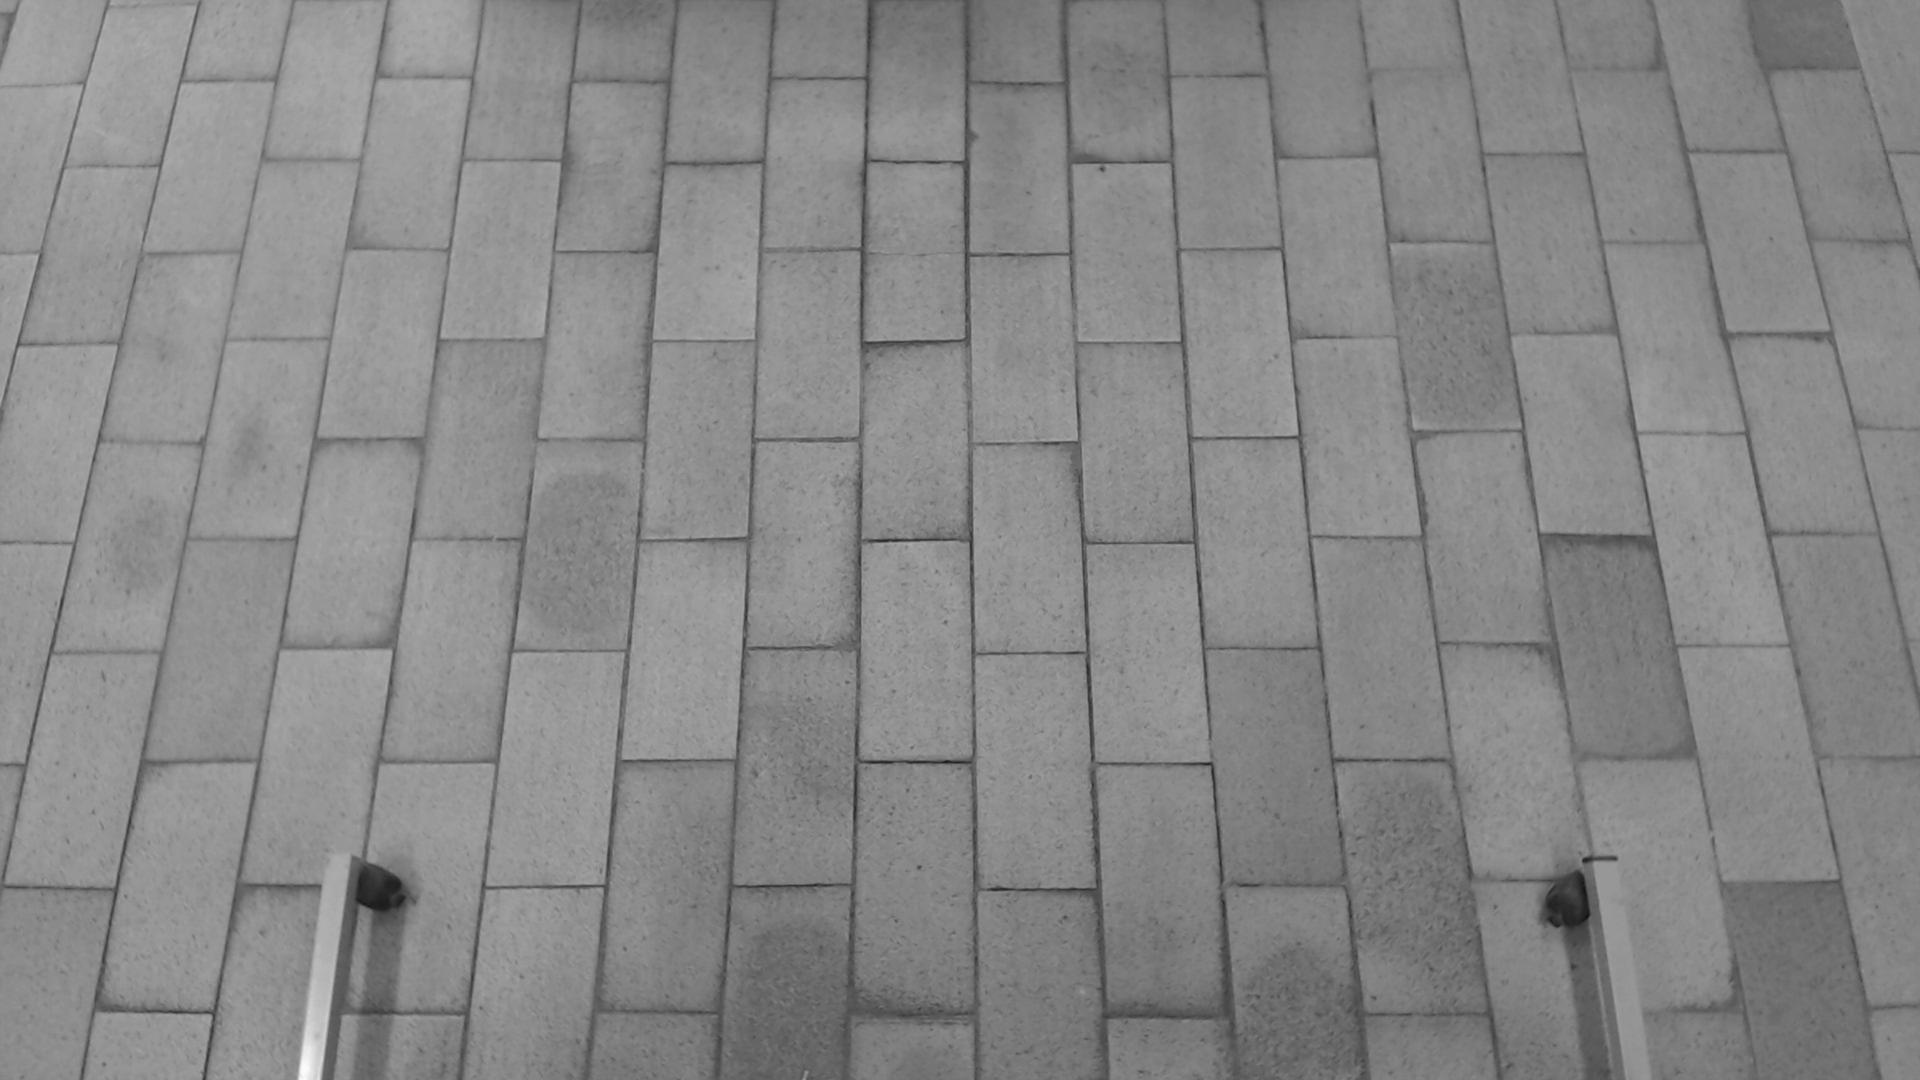
\includegraphics[width=0.32\textwidth]{./figures/LaboratorioBN.jpeg}}
  \subfloat[Modelo \emph{B}]{
   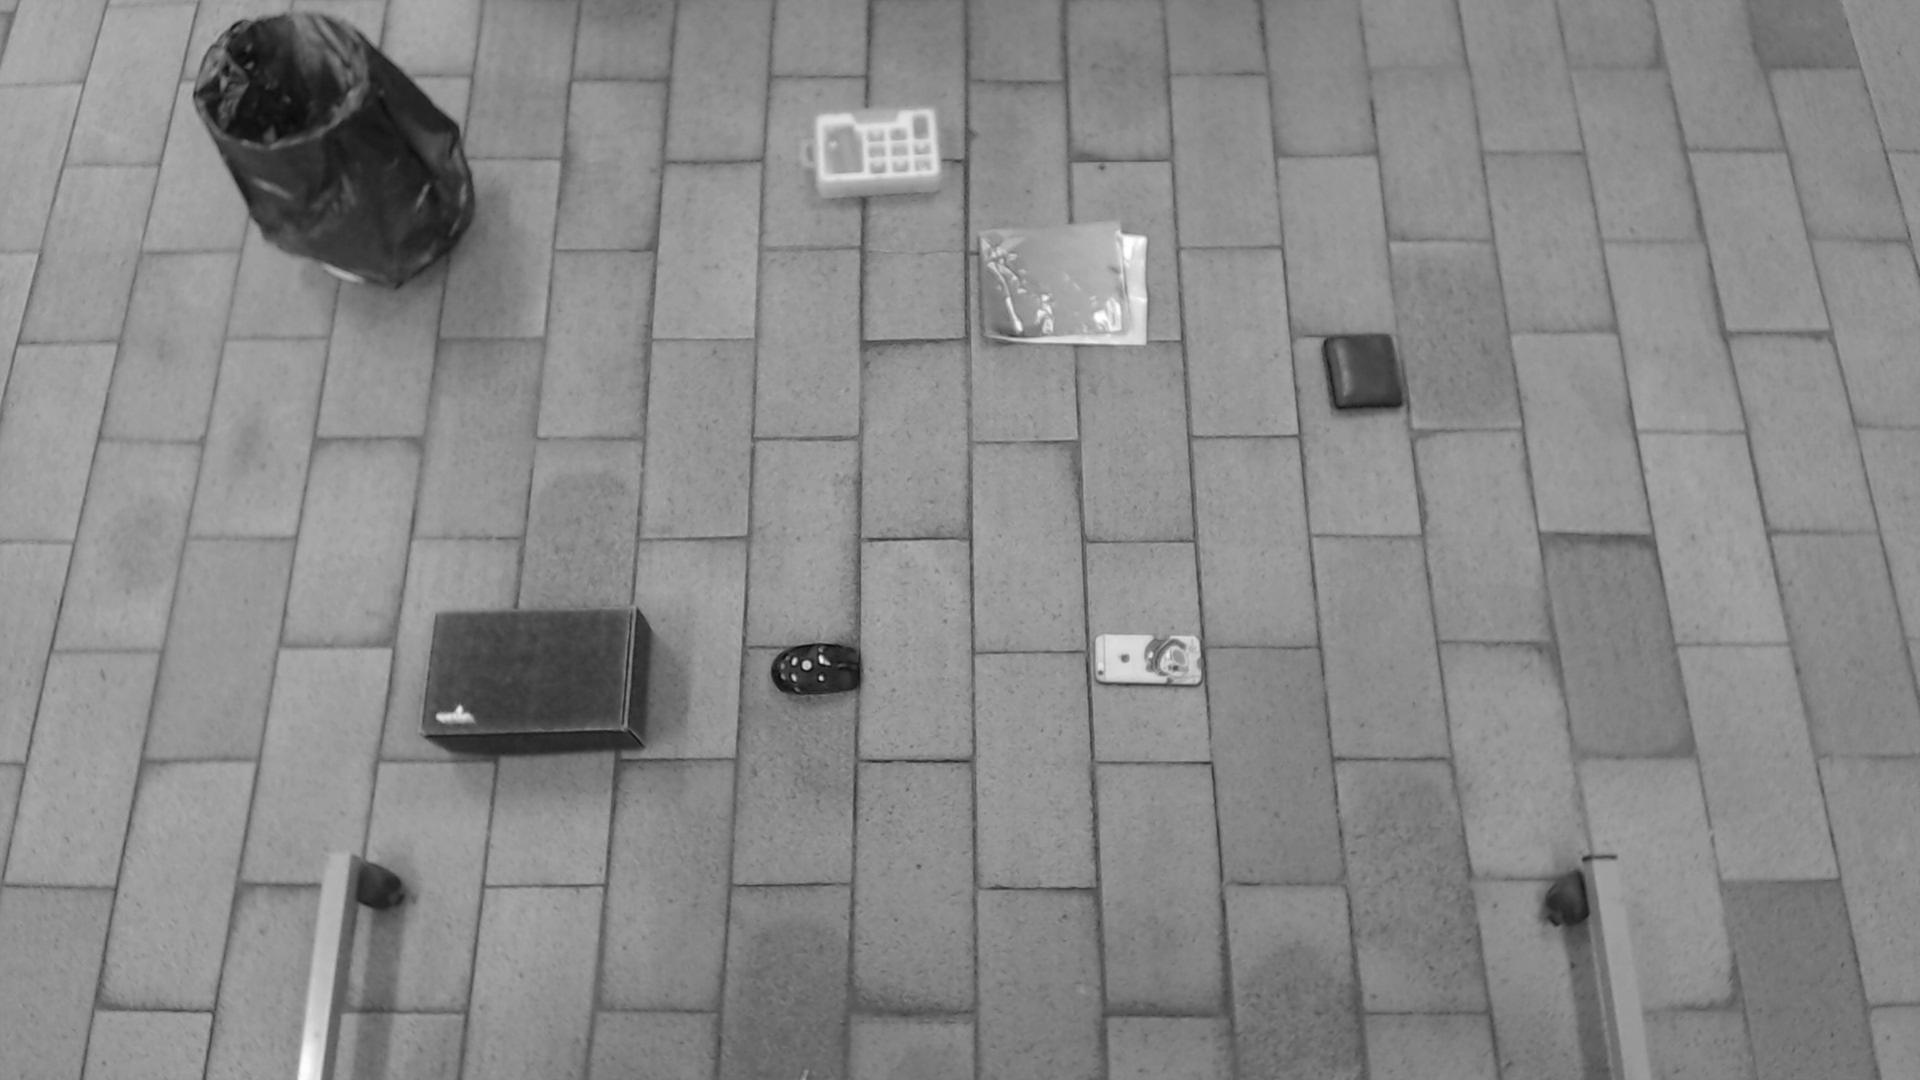
\includegraphics[width=0.32\textwidth]{./figures/LaboratorioObjetosBN.jpeg}}
  \subfloat[Resta imágenes]{
	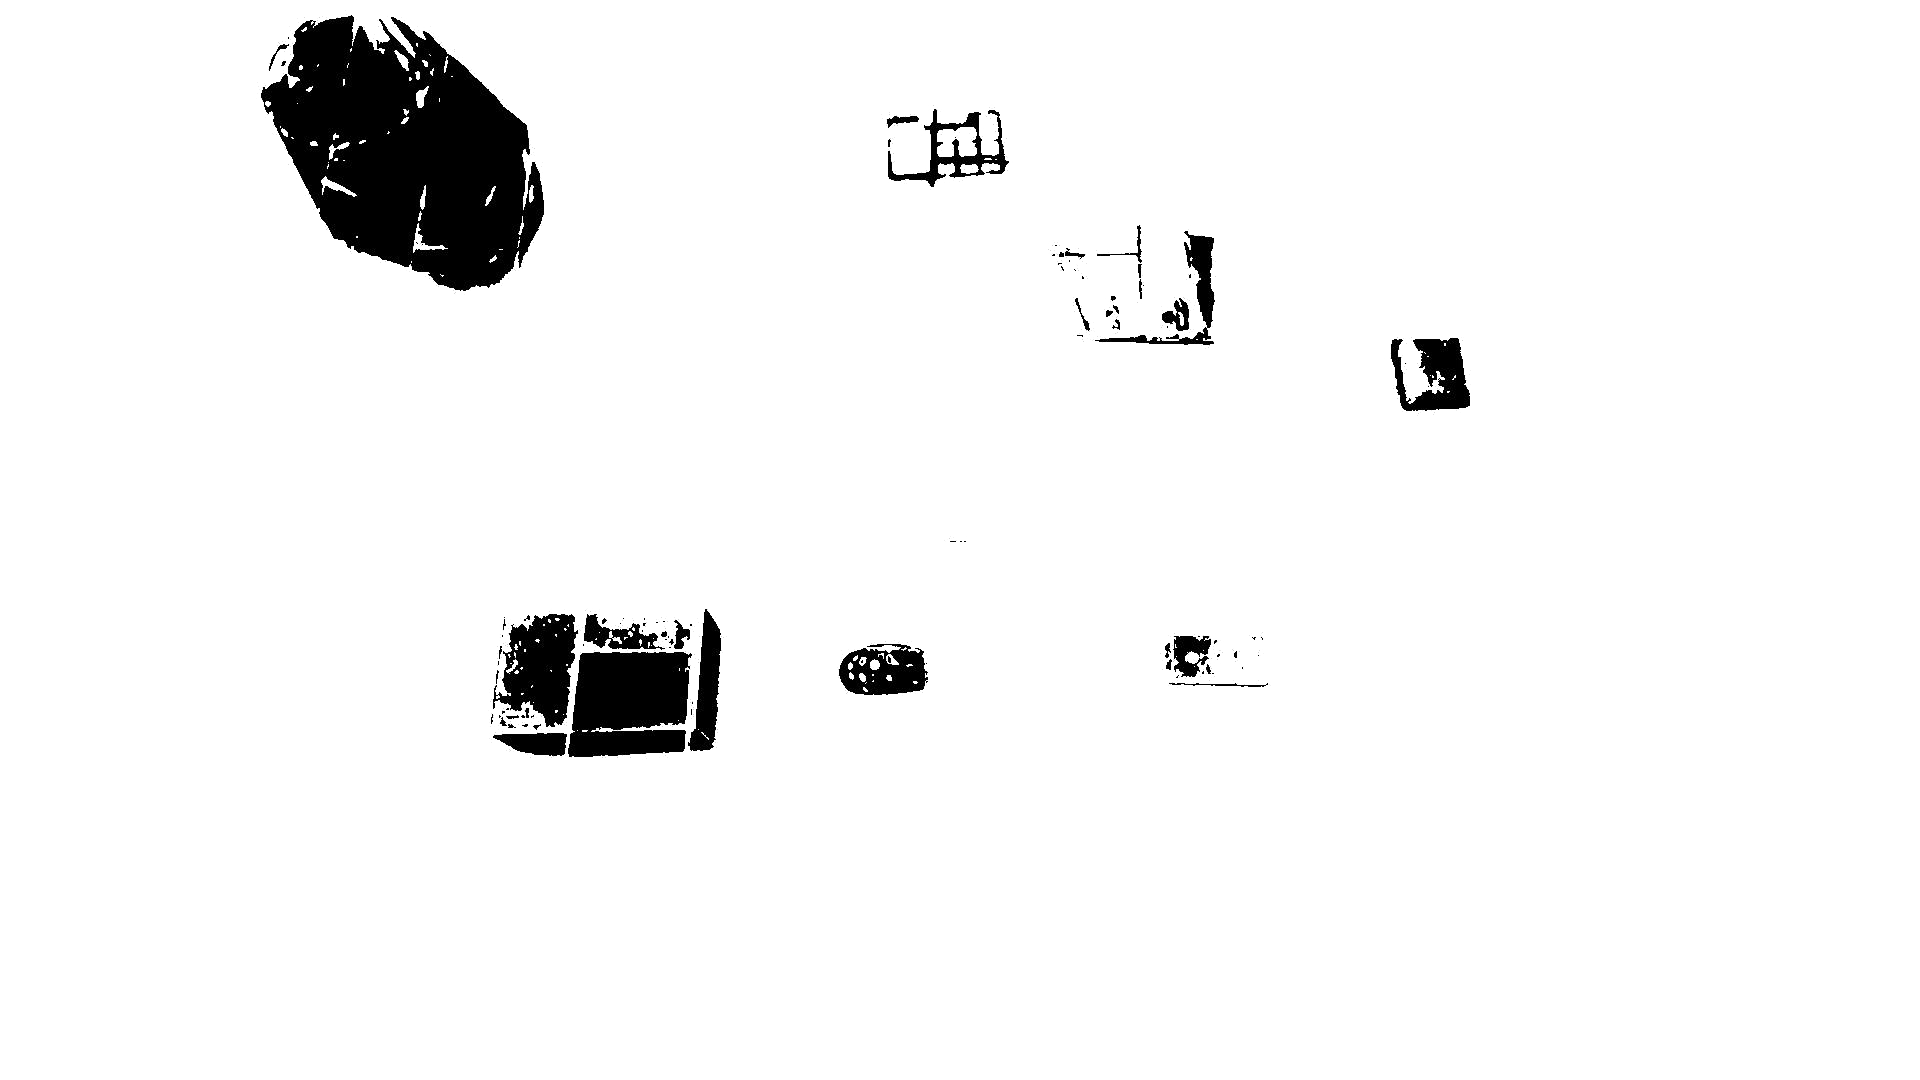
\includegraphics[width=0.32\textwidth]{./figures/RestaObjetos.jpeg}}
 \caption{Ejemplo resta de imágenes}
 \label{fig:DeteccionObjetosLAB}
\end{figure}

\section{Delimitación de los obstáculos}\label{sec:SquareObjetos}

Con tal de evitar que la forma irregular de los objetos pueda dar lugar a que el vehículo colisione con alguno de ellos, se ha decidido implementar un algoritmo que pinte un cuadrado o rectángulo alrededor de los objetos. Para ello, es necesario tomar los 4 puntos más representativos del objeto. el punto superior en la imagen, el punto inferior, el punto más a la izquierda y el punto más a la derecha.

Aunque parezca trivial, es un algoritmo complejo. Estos son los problemas que se han de resolver:

\begin{enumerate}
\item ¿Qué punto representativo corresponde a cada objeto?
\item ¿Cómo guardar la información de forma coherente?
\item ¿La distancia entre dos objetos es menor o igual que el tamaño del vehículo?
\end{enumerate} 

\subsection{¿Qué punto corresponde a cada objeto?}

Para la resolución de este algoritmo se ha decidido recorrer la matriz de datos en dos fases:

\begin{itemize}
\item Fase de análisis
\subitem  Hay que tener en cuenta que por cada iteración se recorre una columna entera de las 1920 posibles. En esta fase se tomará la información acerca de cuántos objetos hay en dicha columna. Si el número de objetos es distinto en comparación con la columna anterior significa que ha comenzado o terminado uno o varios objetos. Como se puede observar hay tres casos posibles referentes al número de objetos:
\begin{enumerate}
\item Que sea menor. Si el número de objetos actual es menor frente al de la columna anterior quiere decir que un objeto ha finalizado. Si se produce esta situación se debe guardar el punto representativo más a la derecha y se debe realizar una comparación tal que si el punto es más alto que en la columna anterior se debe reemplazar por el existente. De manera inversa ocurre lo mismo con el punto inferior ya que si el punto es más pequeño que el guardado anteriormente, se sustituye.
\item Que sea mayor. Si el número de objetos actual es mayor frente al de la columna anterior quiere decir que un objeto nuevo se ha identificado en la matriz de datos. Dado que ha aparecido, se tienen que guardar los valores de los puntos representativos hasta el momento. Es decir, el punto superior e inferior (que pueden ser los mismos en este caso) y el punto más a la izquierda, porque el barrido va de izquierda a derecha. 
\item Que sea igual. Si el número de objetos es el mismo pero es igual a cero, no se realiza ninguna operación. Debido a esto se ha implementado el algoritmo de tal forma que tras la etapa de análisis se comprueba si el número de objetos es mayor que uno, con un contador, y si es así se procede con la fase de resultados. De esta forma evitamos realizar comparaciones con todos los píxeles de la imagen y solo procesamos las columnas que contienen objetos. Si el número es igual pero es mayor que uno, se realiza una comparación entre los valores de los objetos para ver si alguno es mayor o menor que otro punto representativo y merece la pena guardar la información.
\end{enumerate}
\item Fase de resultados
\subitem En esta fase se desplaza el puntero a la derecha por cada iteración y se lleva un orden acerca de dónde se guardan los puntos más representativos de cada objeto.
\end{itemize}

\subsection{¿Cómo guardar la información de forma coherente?}

Cabe mencionar que se ha utilizado un buffer para las coordenadas X y otro buffer para las coordenadas Y, donde se guardará la información que se capture en la fase de análisis para su posterior comparación con los resultados que se guardan en las matrices de resultados para las coordenadas X e Y. Cada objeto posee dos coordenadas X y dos coordenadas Y. Por lo que el primer valor para la coordenada X corresponderá al punto más representativo de la izquierda y el primer valor de la coordenada Y al punto más representativo superior. De tal forma que una vez se hayan examinado las 1920 columnas, se tengan las coordenadas guardadas en las matrices de resultados de las coordenadas X e Y.

Se va a seguir la misma estructura en cuanto a fase de análisis y resultados para explicar cómo se guardan los datos:

\begin{itemize}
\item Fase de análisis
\subitem De igual forma se va a mantener la enumeración acerca de los números de objetos;
\begin{enumerate}
\item Que sea menor. En este caso, si el número de objetos es menor se debe guardar el valor correspondiente a la coordenada X de la columna anterior. Es decir, $x-1$. Así como realizar una comparación con los valores de los puntos representativos superior e inferior por si los valores de la columna anterior son superiores o inferiores respectivamente.
\item Que sea mayor. Si el resultado del número de objetos de la columna actual es mayor que la columna anterior, en primer lugar se debe comprobar si el número de objetos es mayor que uno o igual que uno, debido a que si, por ejemplo, el número de objetos de la columna anterior es uno y el actual dos significa que ha aparecido un nuevo objeto que todavía no se ha terminado de obtener información del objeto que se encuentra en la misma columna a diferente altura. Es por esto, que se debe tener en cuenta el desplazamiento en función del número de objetos ya que sino eliminaríamos valores de objetos que todavía no han terminado de comprobar todos sus puntos. En este caso en concreto se guardaría la coordenada X de la columna actual y las coordenadas Y, aunque tengan el mismo valor, se deben guardar en el punto superior y el punto inferior, ya que posteriormente se irá actualizando.
\item Que sea igual. Si el número de objetos es igual, pero es mayor que cero se debe comprobar el valor de las coordenadas Y, del punto superior e inferior de la coordenada actual por si los valores son más representativos. La información se encuentra en un buffer por lo que el acceso a las coordenadas Y se hace mediante las coordenadas que se han capturado en la fase de análisis y guardado en el buffer. El contador del número de objetos es el que nos servirá para saber a que parte de la matriz debo acceder para consultar la coordenada Y que se ha capturado en la fase de análisis.
\end{enumerate}
\item Fase de resultados
\subitem En la fase de resultados se actualizan los valores de las coordenadas que pasarán a ser las coordenadas de la columna anterior en la siguiente fase de análisis, y se actualizará el buffer con las variables de la coordenada X según el número de objetos que haya habido.

\end{itemize}

\subsection{¿Distancia entre objetos $\leq$ tamaño del vehículo?}

Se va a proceder a describir la parte del algoritmo que controla si la distancia entre dos objetos es menor o igual que el tamaño de vehículo para que se tomen los puntos representativos de los dos objetos en conjunto. Es decir que el cuadrado o rectángulo abarque los dos objetos en uno.

\begin{figure}[bhtp]
 \centering
  \subfloat[Detección de objetos]{
    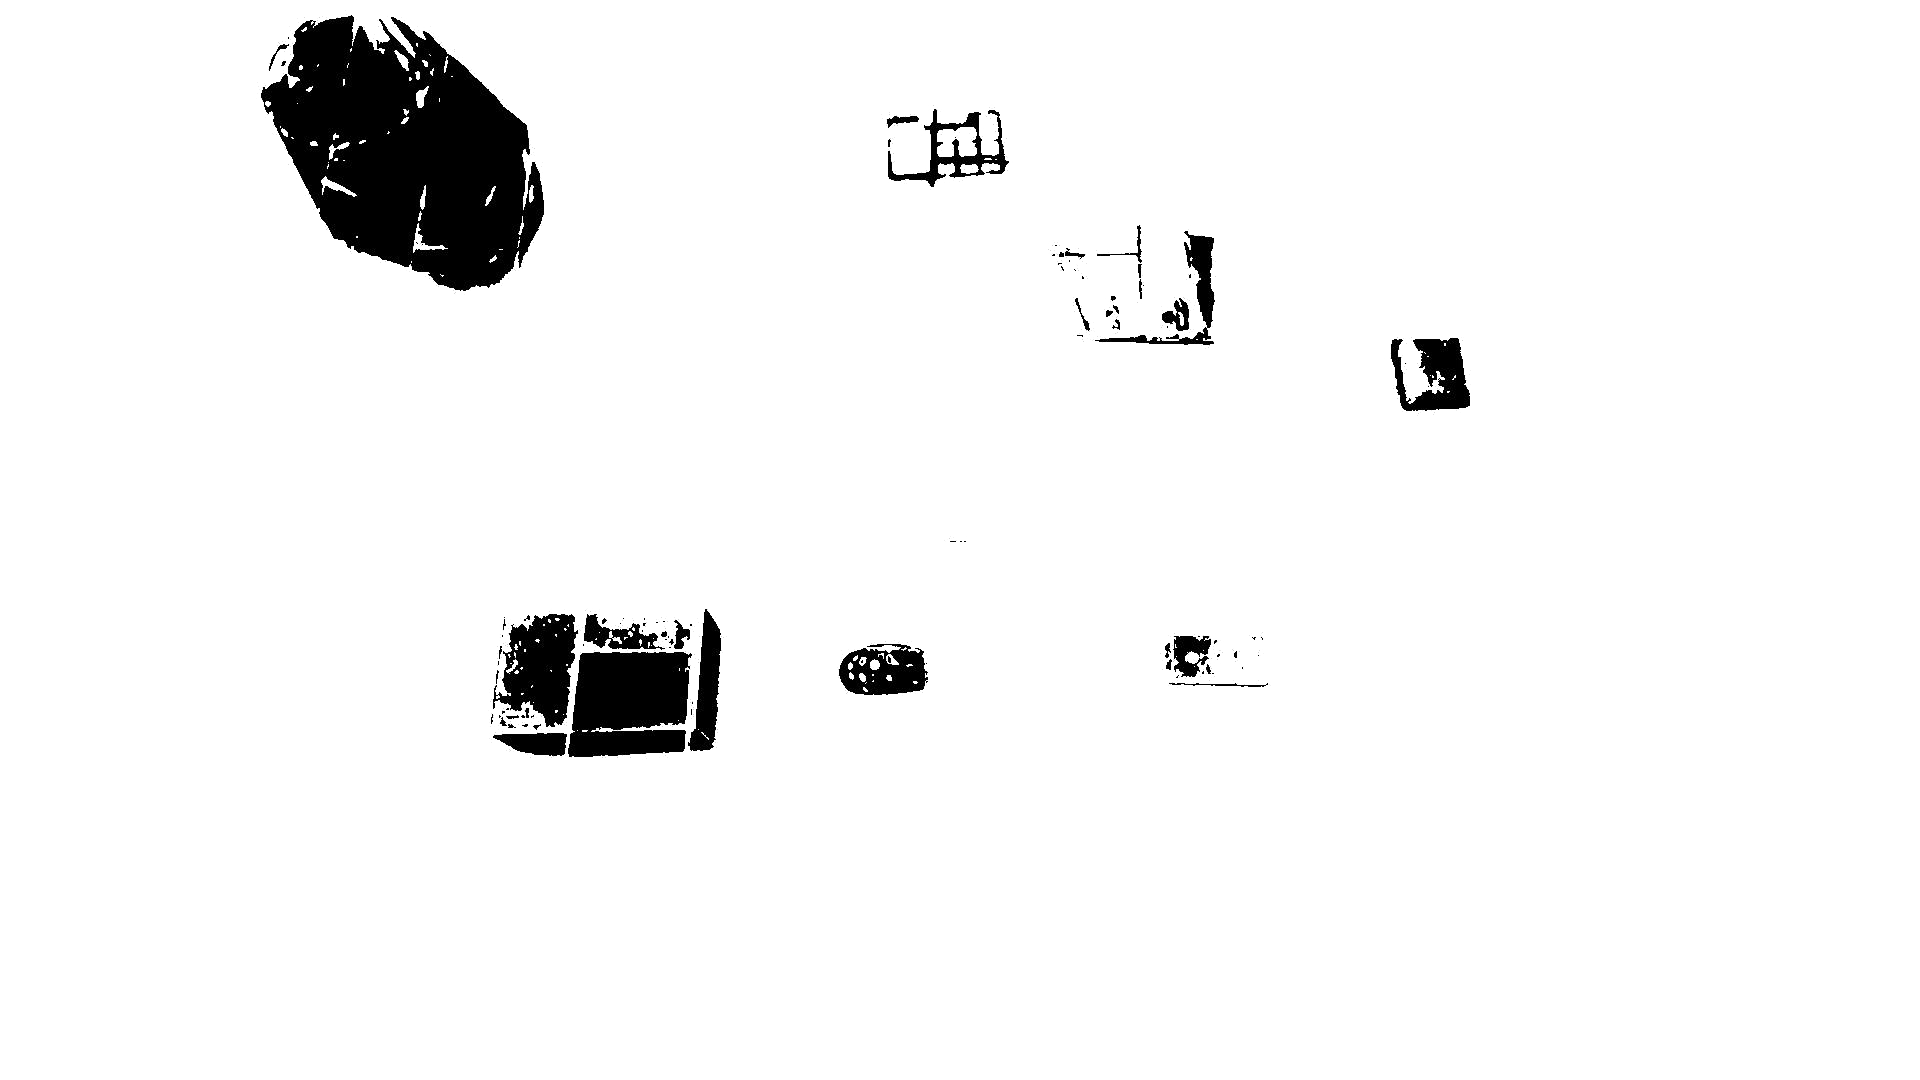
\includegraphics[width=0.49\textwidth]{./figures/RestaObjetos.jpeg}}
  \subfloat[Objetos delimitados]{
    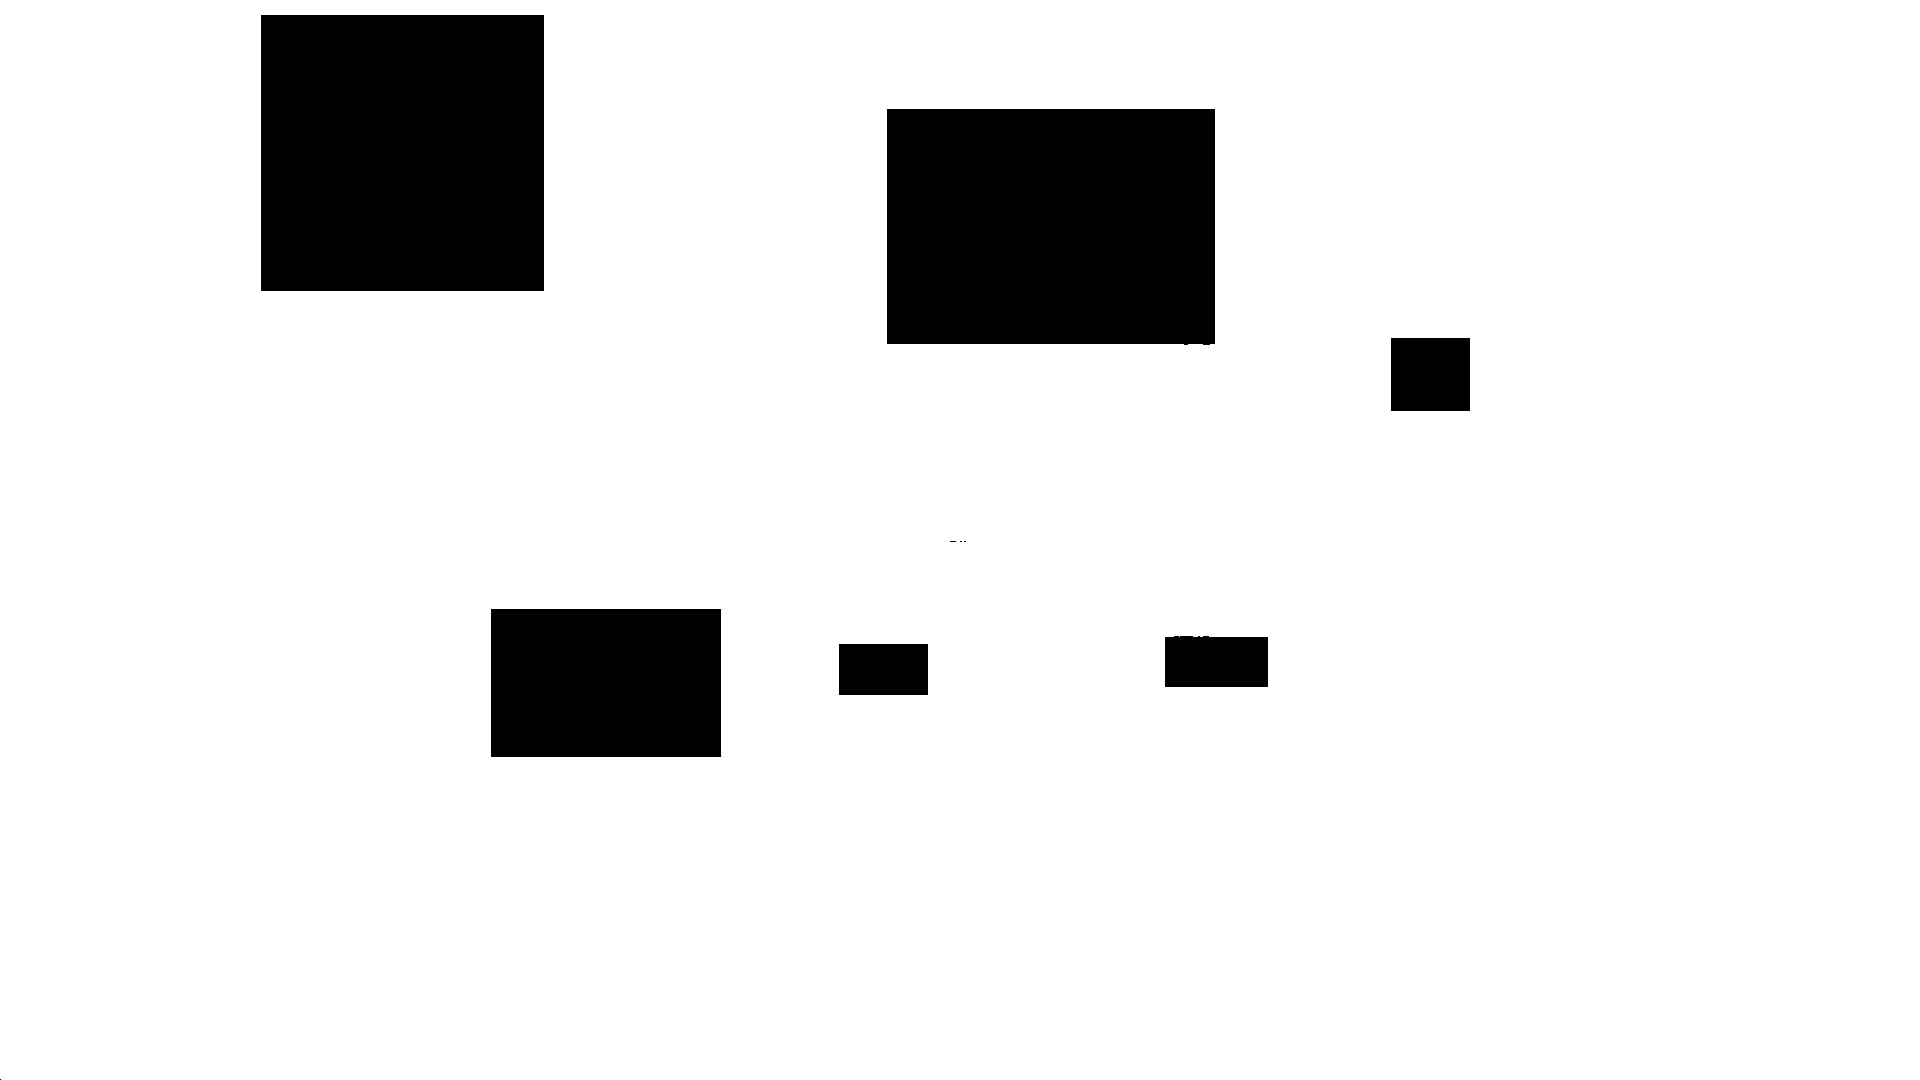
\includegraphics[width=0.49\textwidth]{./figures/CuadradosObjetos.jpeg}}
 \caption{Ejemplo de la delimitación de los obstáculos}
 \label{fig:DetecciónObjetosSquare}
\end{figure}

Para explicar como se ha ido teniendo en cuenta el proceso en concreto de delimitar los objetos, solo se van a utilizar las fases de análisis y resultados a causa de que el número de objetos, salvo que debe ser mayor que uno, no es relevante. 

\begin{itemize}
\item Fase de análisis
\subitem Se va a producir una resta entre el punto inferior más representativo de la coordenada Y del segundo objeto y el punto superior más representativo de la coordenada Y del primer objeto. Si esta resta da un resultado menor que el tamaño del vehículo se guardará el punto inferior más representativo del segundo objeto como el punto superior más representativo del primer objeto. Y el número de objetos se decrementará en uno. El procedimiento es el mismo para un número de objetos mayor.
\item Fase de resultados
\subitem En esta fase se va a realizar el mismo tipo de cálculo que en la fase de análisis, pero esta vez con las coordenadas X. Si el número de objetos es mayor que uno se realizará una resta entre el punto más a la izquierda del segundo objeto y el punto más a la derecha del primer objeto. Si el resultado de esta operación es menor que el tamaño del vehículo, se modificará el punto más a la derecha del primer objeto por el punto representativo más a la izquierda del segundo objeto. Y también se decrementará en uno el número de objetos. 
\end{itemize}

\section{Implementación del algoritmo A* en \emph{C++}, sin restricciones}\label{sec:AEstrellaSoftware}

Se ha decidido utilizar el algoritmo de A* debido a que es un algoritmo que calcula la ruta óptima realizando un número de operaciones menor que otro tipo de algoritmos clásicos como Djikstra o \ac{BFS}. Se han realizado un número de pruebas acerca de los resultados obtenidos de estos tres algoritmos y estos han sido los resultados para el mismo caso de estudio. 

\begin{figure}[bhtp]
 \centering
  \subfloat[Algoritmo A* Longitud = 14 ,Tiempo = 1.2 ms, Operaciones: 114 ]{
    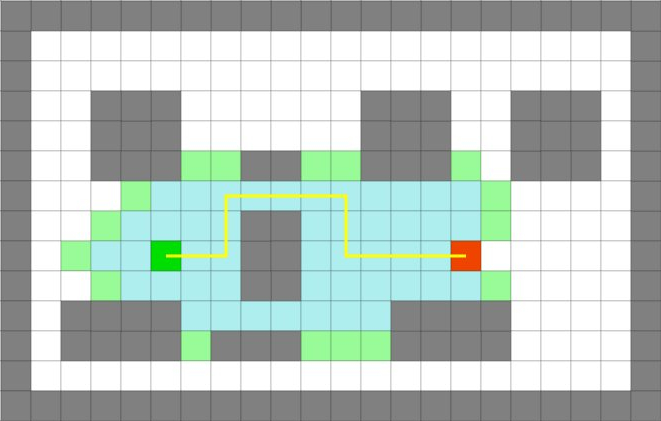
\includegraphics[width=0.33\textwidth]{./figures/AEstrella-4DIR.jpeg}}
  \subfloat[BFS:  Longitud = 14 ,Tiempo = 1.4 ms, Operaciones: 277 ]{
    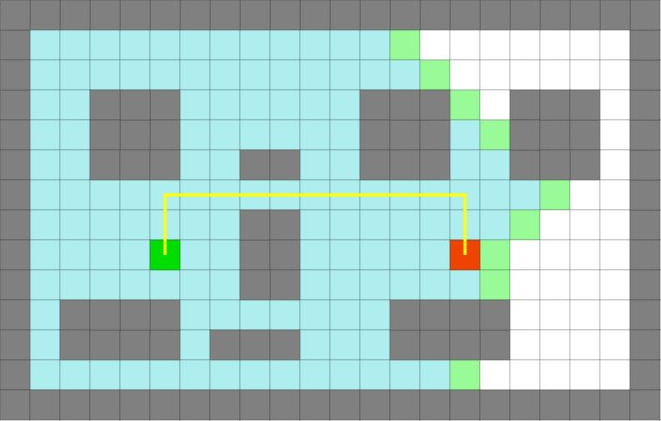
\includegraphics[width=0.33\textwidth]{./figures/BFS-4DIR.jpeg}}
  \subfloat[Djikstra: Longitud = 14 ,Tiempo = 5.0 ms, Operaciones: 274]{
    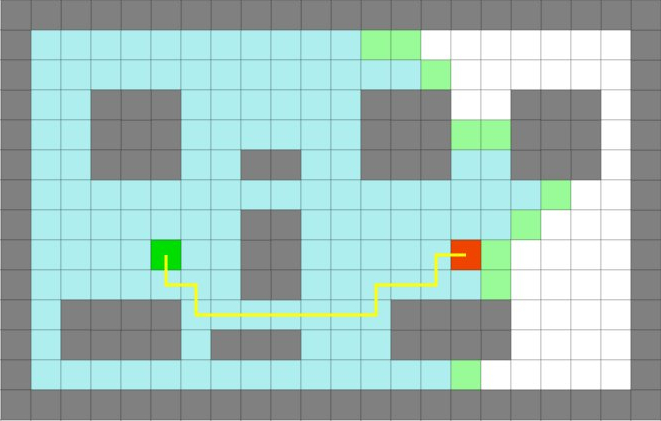
\includegraphics[width=0.33\textwidth]{./figures/Dijkstra-4DIR.jpeg}}
 \caption{Casos de prueba con 4 Direcciones}
 \label{fig:DetecciónObjetosSquare}
\end{figure}

\begin{figure}[bhtp]
 \centering
  \subfloat[Algoritmo A* Longitud = 11.7 ,Tiempo = 3.6 ms, Operaciones: 68 ]{
    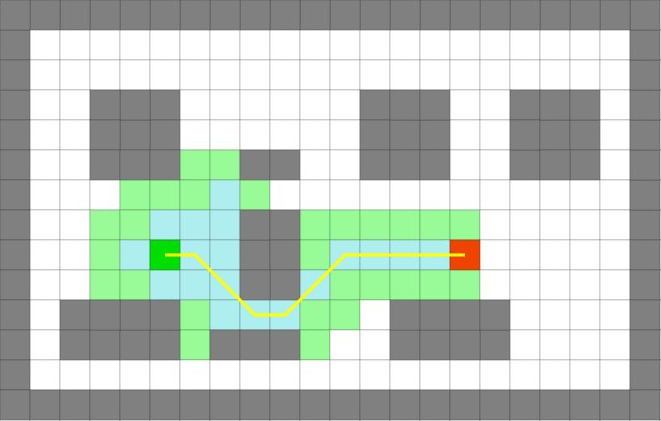
\includegraphics[width=0.33\textwidth]{./figures/AEstrella-8DIR.jpeg}}
  \subfloat[BFS:  Longitud = 11.7 ,Tiempo = 1.7 ms, Operaciones: 273 ]{
    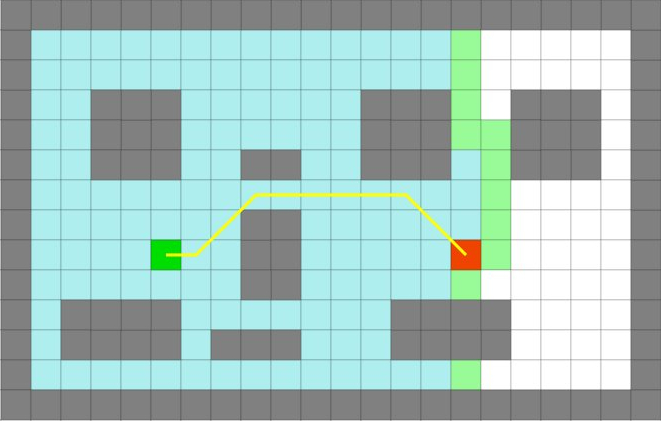
\includegraphics[width=0.33\textwidth]{./figures/BFS-8DIR.jpeg}}
  \subfloat[Djikstra: Longitud = 11.7 ,Tiempo = 3.5 ms, Operaciones: 270]{
    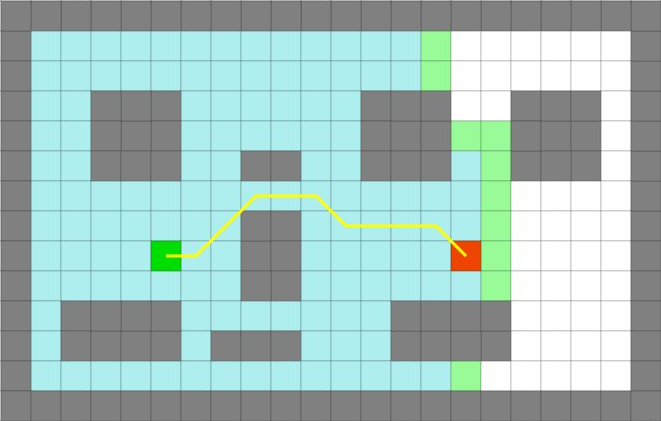
\includegraphics[width=0.33\textwidth]{./figures/Dijkstra-8DIR.jpeg}}
 \caption{Casos de prueba con 8 Direcciones}
 \label{fig:DetecciónObjetosSquare}
\end{figure}

Para esta iteración, el objetivo principal es conseguir que funcione el algoritmo de cálculo de trayectoria A*. Se ha utilizado de base una implementación realizada en el lenguaje \emph{C++} \cite{ImplementacionAlgoritmoA}. Con la modificación de esta implementación para que los datos que se utilizan como argumento sean los que se han calculado previamente en la detección de los obstáculos se ha podido calcular la trayectoria teórica por la que debe avanzar el vehículo.

\section{Detección del vehículo frente a los objetos}\label{sec:DeteccionVehiculo}

Para distinguir el vehículo del resto de objetos del escenario se ha decidido utilizar una combinación de algoritmos de la librería \emph{OpenCV}. En primer lugar se utiliza la función \emph{cvtColor} que nos permite tranformar una imagen en modelo de color \acx{RGB} a \acx{HSV}\footnote{El modelo de color \ac{HSV} es una transformación no lineal del modelo \ac{RGB} en coordenadas cilíndricas de manera que cada color viene definido por el tinte o matiz, saturación y brillo.}. Se ha decidido utilizar el modelo de color \ac{HSV} ya que nos permite identificar un color por un solo valor, el matiz, en lugar de tres valores como en el modelo de color \ac{RGB}. Con el uso de la función \emph{cvtColor} y la función \emph{inRange} se puede seleccionar el umbral de color que se quiera obtener de la imagen de referencia. Por ejemplo, el color rojo en \emph{OpenCV} tiene el valor del matiz entorno al rango de 0 a 10 y de 160 a 180. Con el uso de estas dos funciones, configuradas para detectar objetos de color rojo, se obtienen los resultados de la figura \ref{fig:CirculosDetectados}.

\begin{figure}[hbtp]
 \centering
  \subfloat[Imagen Original]{
    
\includegraphics[width=0.4\textwidth]{./figures/Circulos.jpeg}}
  \subfloat[Imagen Resultado]{
    
\includegraphics[width=0.4\textwidth]{./figures/CirculosDetectados.jpeg}}
 \caption{Ejemplo de uso con las funciones \emph{cvtColor} y \emph{inRange}}
 \label{fig:CirculosDetectados}
\end{figure}

Debido a que se puede dar la situación en la que haya dos objetos de color rojo, se ha decidido utilizar la función \emph{HoughCircles} que detecta los círculos en una imagen, de tal manera que en el caso de que haya figuras diferentes con el mismo color solo detecte las que tengan forma circular. Como aparece en la imagen \ref{fig:CirculosRojosDetectados}. Esta funcionalidad es muy útil, ya que si se define un umbral de color reducido para el matiz y se pone una marca circular identificativa al vehículo con el color perteneciente al umbral, se puede diferenciar el vehículo del resto de objetos con facilidad.

\begin{figure}[htbp]
 \centering
  \subfloat[Imagen Original]{
    
\includegraphics[width=0.4\textwidth]{./figures/CirculosRojosOriginal.jpeg}}
  \subfloat[Imagen Resultado]{
    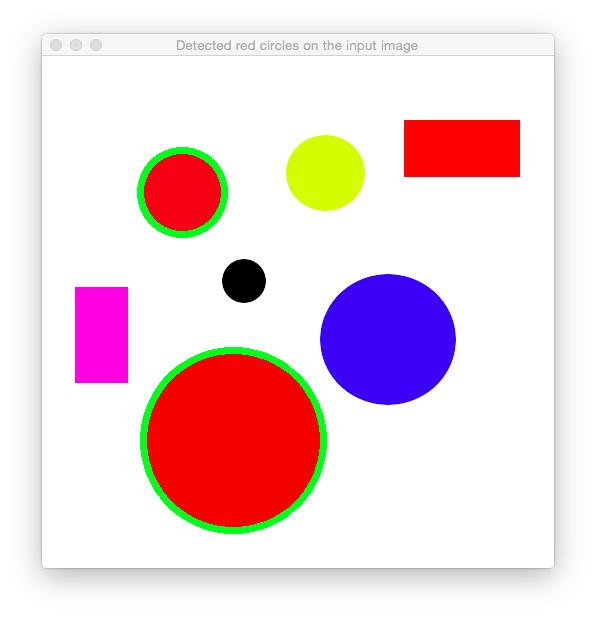
\includegraphics[width=0.4\textwidth]{./figures/CirculosRojosDetectados.png}}
 \caption{Uso de las funciones \emph{cvtColor}, \emph{inRange} y \emph{HoughCircles}}
 \label{fig:CirculosRojosDetectados}
\end{figure}

Además, con la función \emph{Pointcenter} se pueden obtener las coordenadas del punto central del círculo. Esta funcionalidad es muy útil ya que para poder inicializar el algoritmo de cálculo de trayectoria es necesario conocer las coordenadas en las que se encuentra el vehículo. Por ello, mediante el uso combinado de las cuatro funciones mencionadas anteriormente, se puede diferenciar el coche del resto de objetos del escenario mediante la detección de la marca circular identificativa de color rojo, así como obtener las coordenadas en las que se encuentra el vehículo para poder llevar a cabo la ejecución del algoritmo de cálculo de trayectoria.



\section{Diseño del vehículo del sistema}\label{sec:DiseñoVehiculo}

Como brazo ejecutor del sistema se ha decidido integrar una serie de componentes con los cuales se pueda llevar a cabo la conducción, comunicación, y traducción de la información en movimientos. A continuación se va a proceder a nombrar los elementos que forman el vehículo:

\begin{itemize}
\item \emph{Arduino} UNO R3 ATMEGA328
\item Controlador \emph{Sparkfun} Ardumoto
\item Chasis con motores de corriente continua de 9V.
\item Módulos \emph{Xbee} de la marca \emph{Digi}.
\item Batería recargable \emph{Odec} 9V.
\item Placa de pruebas \emph{Arduino}.
\item \emph{Arduino} Shield. 
\item Sensor efecto Hall A3144.
\end{itemize}

Si desea conocer más acerca del porqué del uso de estos componentes puede echar un vistazo en el anexo \ref{anexo:Codigo}.

\section{Comunicación con el vehículo}\label{sec:Comunicacion}

Para establecer la comunicación entre la placa \emph{Zedboard} y la placa del coche \emph{Arduino UNO} se ha decidido utilizar una pareja de módulos XBee\footnote{Los chips Xbee son capaces de comunicarse de forma inalámbrica unos con otros.} de la marca \emph{Digi} \cite{Digi}. Mediante estos chips de conexión inalámbrica podemos establecer una comunicación serial sin necesidad de conectarlos por cable. Esta opción es muy interesante debido a que mediante el software \emph{XCTU}\footnote{XCTU \cite{XCTU} es una aplicación multi-plataforma, gratuita, que incluye herramientas que facilitan la instalación, configuración y prueba de funcionamiento entre módulos XBee a través de una interfaz gráfica fácil de usar.} que proporciona la marca \emph{Digi} se puede establecer una comunicación punto a punto entre las dos placas del sistema de una forma rápida y sencilla.

Ahora bien, debido a la importancia que tiene que se realicen todas las órdenes de forma ordenada y secuencial, es necesario establecer un protocolo de comunicación mediante el cual se controle que no se pierde ni se corrompe ningún paquete de información.

Dado que el sistema está pensado para funcionar en tiempo real, se ha decidido implementar un protocolo específicamente pensado para este \ac{TFG} de tal forma que se optimice el tamaño de datos que se envían. Se controle mediante \acx{ACK} que los paquetes de información han llegado y se comunique si ha habido algún error en la ejecución del movimiento. 

\subsection{Protocolo de comunicación}\label{subsec:Protocolo}

Debido a que se ha diseñado un vehículo que ejecuta sus movimientos accionando dos motores independientes entre si de corriente continua, sin encoder lineal\footnote{Un encoder lineal es un dispositivo o sensor que cuenta con una escala graduada para determinar su posición. Los sensores en el encoder leen la escala para después convertir su posición codificada en una señal digital que puede ser interpretada por un controlador de movimiento electrónico.}, la distancia a recorrer se traducirá en números de vueltas a ejecutar por las ruedas del vehiculo. Para ello, los paquetes de información a transmitir poseeran los siguientes campos:

\begin{itemize}
\item Identificador de la orden que se debe ejecutar. 

Se ha decidido utilizar un byte para identificar la orden a ejecutar. El sistema genera cada orden con un número identificador de manera secuencial, no genera un nuevo movimiento hasta que sepa el estado final de la comunicación que ha realizado previamente. Por ello, no se puede dar lugar la situación en la que se comuniquen dos movimientos distintos que tengan el mismo identificador.% porque el número de movimientos necesarios sea mayor que 256.
\item La dirección que debe tomar el vehículo.

Según se ha diseñado, el vehículo puede tomar cualquiera de las 8 direcciones de los puntos cardinales. Por ello, se ha decidido asignar 3 bits con los cuales se pueden representar las 8 posibles direcciones. No es necesario especificar que el vehículo frene ya que si no se realiza ninguna orden, el vehículo no acciona ningún motor.
\item El número de vueltas que deben realizar las ruedas del vehículo.

La cámara cenital se puede encontrar fija a distintas alturas, por lo que la distancia real que corresponde a cada píxel puede variar. Ya que cuanto más lejos esté la cámara del suelo, mayor será la distancia real que exista entre dos píxels de una imagen. Por ello, se ha decidido asignar un nuevo byte más el resto de bits del segundo byte en el que se encuentran los tres bits que representan la dirección que debe tomar el vehículo. Con lo cual, el número de bits que se utilizan para representar el número de vueltas que deben realizar las ruedas del vehículo son 13. 
\end{itemize}

De esta forma, cada paquete tendrá un tamaño fijo de tres bytes. A continuación se va a proceder a exponer un ejemplo de cómo funciona el protocolo de comunicación.

\subsection{Ejemplo de funcionamiento del protocolo de comunicación}\label{subsec:EjemploProtocolo}

Se ha decidido diseñar un escenario de prueba con el cual se pueda explicar cómo funciona en detalle el protocolo de comunicación que se ha implementado. Para ello, se ha generado un diagrama de secuencia, figura \ref{fig:DiagramaSecuencia}, en el cual se representa la comunicación que se establece entre la placa \emph{Zedboard} y \emph{Arduino}. Para evitar desarrollar un escenario muy extenso, se va a representar un ejemplo aleatorio de 4 peticiones de movimiento. Se contemplará la opción de que se pierda información en la comunicación para representar los posibles inconvenientes que se pueden dar lugar en la ejecución del sistema en tiempo real. 

Posteriormente, se va a proceder a explicar cómo está estructurada la información de los paquetes que se desean comunicar. Ya que como se ha optimizado el tamaño, existen tres conjuntos de bits que representan los parámetros mencionados en la subsección \ref{subsec:Protocolo}.

\begin{figure}[hbtp]
\centering
	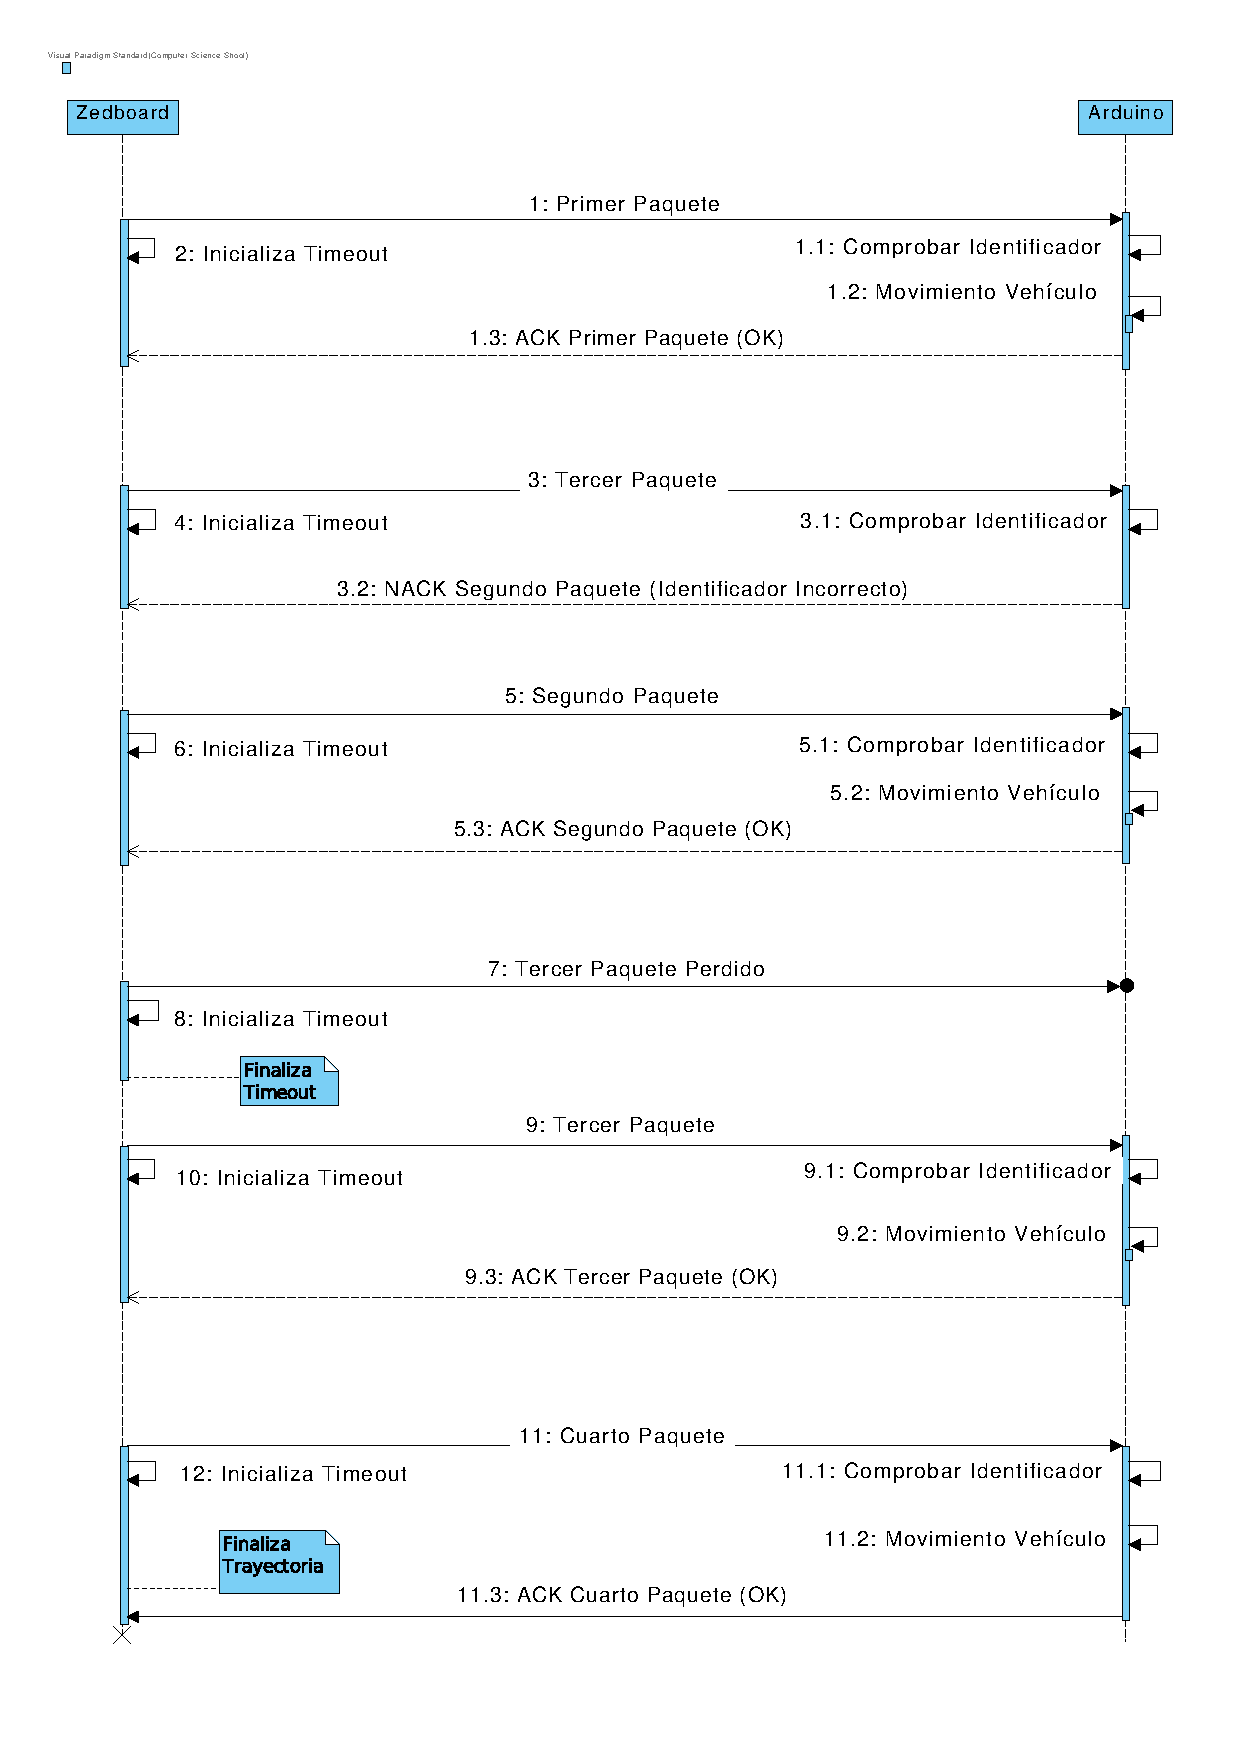
\includegraphics[width=1\textwidth]{./figures/DiagramaSecuencia.pdf}
	\caption{Diagrama de secuencia del protocolo de comunicación}
	\label{fig:DiagramaSecuencia}
\end{figure}

Se pueden distinguir tres bloques fijos por paquete que representan los bytes, aunque la información está estructurada tal como representan los colores:

\begin{itemize}
\item Morado: Representa los 8 primeros bits en los cuales se desea transmitir el identificador numérico de la trama\footnote{En redes, una trama es una unidad de envío de datos. Es una serie sucesiva de bits, organizados en forma cíclica, que transportan información y que permiten en la recepción extraer esta información.} con el que se desea comprobar si la comunicación se está realizando de forma secuencial y ordenada. Como utilizamos 8 bits para representar el identificador estos valores estarán entre 0 y 255.
\item Rojo: Representa los 3 primeros bits del segundo byte de la trama. Esta información se utilizará para activar los motores del vehículo de tal forma que se mueva en la dirección que interese.% Es decir, al haber tres bits, el vehículo podrá tomar la dirección de cualquiera de los 8 puntos cardinales.
\item Negro: Representa los 5 últimos bits del segundo byte y los 8 bits del tercer byte de la trama. En total se utilizan 13 bits para representar el número de vueltas que deben realizar las ruedas del vehículo para completar la orden.
\end{itemize}

%\begin{table}[hbtp]
%\centering
%\begin{tabular}{|l|l|}
%\hline
%\rowcolor[HTML]{9B9B9B}
%\multicolumn{2}{|c|} {\textbf{Direcciones}}\\ \hline
%{\color[HTML]{FF0000} \textbf{000}} &  Delante\\ \hline
%{\color[HTML]{FF0000} \textbf{001}} &  Diagonal Superior derecha\\ \hline
%{\color[HTML]{FF0000} \textbf{010}} &  Derecha\\ \hline
%{\color[HTML]{FF0000} \textbf{011}} &  Diagonal inferior derecha\\ \hline
%{\color[HTML]{FF0000} \textbf{100}} &  Detras\\ \hline
%{\color[HTML]{FF0000} \textbf{101}} &  Diagonal inferior izquierda\\ \hline
%{\color[HTML]{FF0000} \textbf{110}} &  Izquierda\\ \hline
%{\color[HTML]{FF0000} \textbf{111}} &  Diagonal superior izquierda \\ \hline
%\end{tabular}
%\caption{Tabla de direcciones del vehículo en bits}
%\label{tab:Direcciones}
%\end{table}

A continuación se va a proceder a explicar el diagrama de secuencia, de la figura \ref{fig:DiagramaSecuencia}, con la información detallada de cada paquete.

\begin{enumerate}

\item Primer paquete
\begin{figure}[hbtp]
\centering
	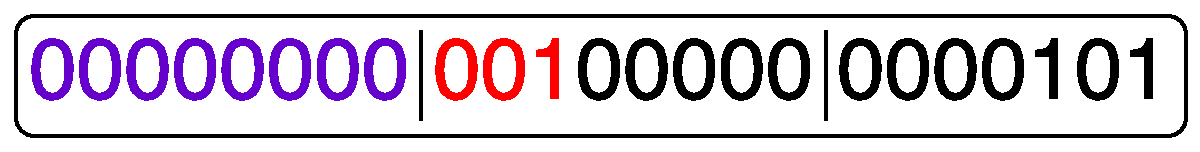
\includegraphics[width=.9\textwidth]{./figures/Comunicacion1.pdf}
	\label{fig:Comunicacion1}
\end{figure}

Se produce el envío del primer paquete desde la placa \emph{Zedboard} para que se realice un movimiento de 5 vueltas hacia la diagonal superior derecha, según la tabla \ref{tab:Direcciones}. Una vez se ha realizado el envío se inicializa el timeout del puerto serie de la placa \emph{Zedboard}. 

Desde la placa \emph{Arduino} se comprueba si el identificador coincide con el número de paquete que se desea recibir. Como se espera recibir el paquete con el identificador 0, se procede a llamar al método que activa los motores para avanzar hacia la diagonal superior izquierda. Una vez se han realizado las 5 vueltas, \emph{Arduino} devuelve un ACK a la placa \emph{Zedboard} confirmando que se ha realizado el movimiento correctamente  y finaliza la comunicación del primer paquete.

 % FIN CASO 1

\item Segundo paquete
\begin{figure}[hbtp]
\centering
	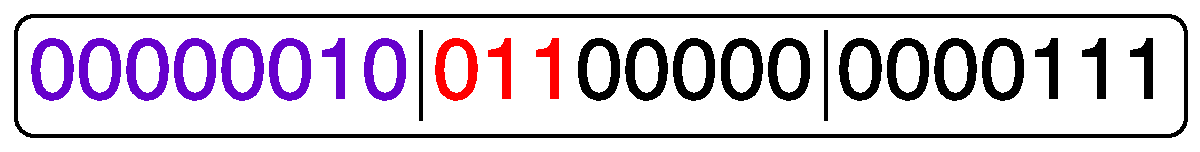
\includegraphics[width=.9\textwidth]{./figures/Comunicacion3.pdf}
	\label{fig:Comunicacion1}
\end{figure}

Debido a un error en el sistema, se procede a enviar el paquete que corresponde al identificador del tercer movimiento. Como la placa \emph{Arduino} tiene un contador propio, para llevar el control acerca de que paquete espera, detecta que el paquete que está recibiendo desde la placa \emph{Zedboard} no contiene la información correspondiente al segundo movimiento. Por ello, tras realizar la comprobación del identificador genera un NACK que envía a la placa \emph{Zedboard} para comunicar que está esperando la información que corresponde al segundo movimiento. De esta forma se termina la comunicación del paquete incorrecto y se genera un nuevo paquete con la información correspondiente al identificador que espera.

Una vez se ha generado el paquete correspondiente al segundo movimiento, se envía la información y el software de \emph{Arduino} realiza el movimiento de una vuelta hacia la derecha, enviando un ACK a la placa \emph{Zedboard} cuando finaliza el movimiento. 

% FIN CASO 2

\item Tercer paquete
\begin{figure}[hbtp]
\centering
	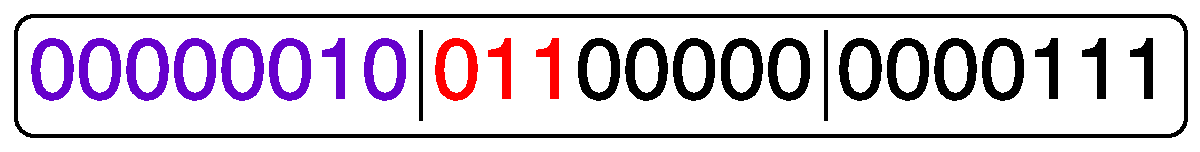
\includegraphics[width=.9\textwidth]{./figures/Comunicacion3.pdf}
	\label{fig:Comunicacion1}
\end{figure}

La placa \emph{Zedboard} envía la información correspondiente al tercer movimiento por el puerto serie. Pero debido a las interferencias que se encuentran en el escenario, este paquete nunca llega a la placa \emph{Arduino}. Como consecuencia, el timeout que se ha definido en el puerto serie, de la placa \emph{Zedboard}, llega a su fin y genera una interrupción que finaliza la comunicación correspondiente al paquete del tercer movimiento.

Dado que el tercer movimiento no se ha realizado, se vuelve a enviar el paquete por el puerto serie. Esta vez la información si que llega a la placa \emph{Arduino} realizando un movimiento de 8 vueltas de rueda hacia la dirección diagonal inferior derecha.

% FIN CASO 3

\item Cuarto paquete
\begin{figure}[hbtp]
\centering
	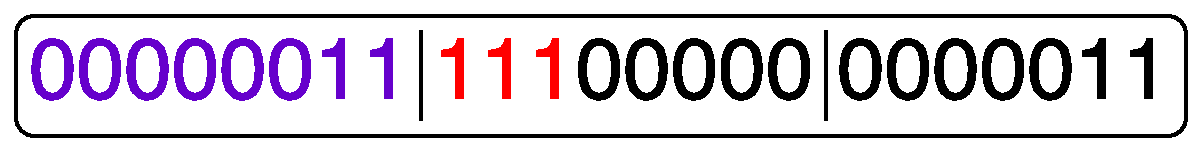
\includegraphics[width=.9\textwidth]{./figures/Comunicacion4.pdf}
	\label{fig:Comunicacion1}
\end{figure}

Por último, se realiza el envío por el puerto serie correspondiente al cuarto movimiento. Que tras llegar sin problemas realiza un movimiento de tres vueltas de rueda hacia la dirección diagonal superior izquierda. Como en este ejemplo solo se realizan cuatro movimientos, el programa encargado de coordinar la comunicación, desde la placa \emph{Zedboard}, finaliza el proceso.

% FIN CASO 4

\end{enumerate} %FIN ENUMARATE

\subsection{Maqueta de pruebas del protocolo de comunicación}\label{MaquetaPruebas}

Se ha diseñado una maqueta para poder comprobar el funcionamiento del protocolo de comunicación previamente a su instauración en el sistema. De esta forma se puede probar el funcionamiento del protocolo de una manera más eficiente en la etapa de desarrollo. Utilizar una maqueta de pruebas proporciona las siguientes ventajas al programador:

\begin{itemize}
\item Evita problemas ajenos al funcionamiento del protocolo de comunicación. Debido a que esta maqueta está desarrollada exclusivamente para emular la comunicación entre la placa \emph{Zedboard} y \emph{Arduino}. Se evita que errores que se puedan deber al funcionamiento de otros algoritmos enturbien el desarrollo del protocolo.
\item Elude utilizar más recursos de los necesarios. De esta forma se evita perder tiempo en la configuración de la placa \emph{Zedboard}, ya que mediante la utilización del puerto serie del ordenador, en el cual implementamos el código, es suficiente para poder comprobar el funcionamiento de la comunicación. 
\item Reduce el tiempo de diseño.
\end{itemize}

A continuación se va a proceder a explicar el funcionamiento de la maqueta aplicado al protocolo de comunicación.

\subsubsection{Funcionamiento de la maqueta}

\begin{figure}[hbtp]
\centering
	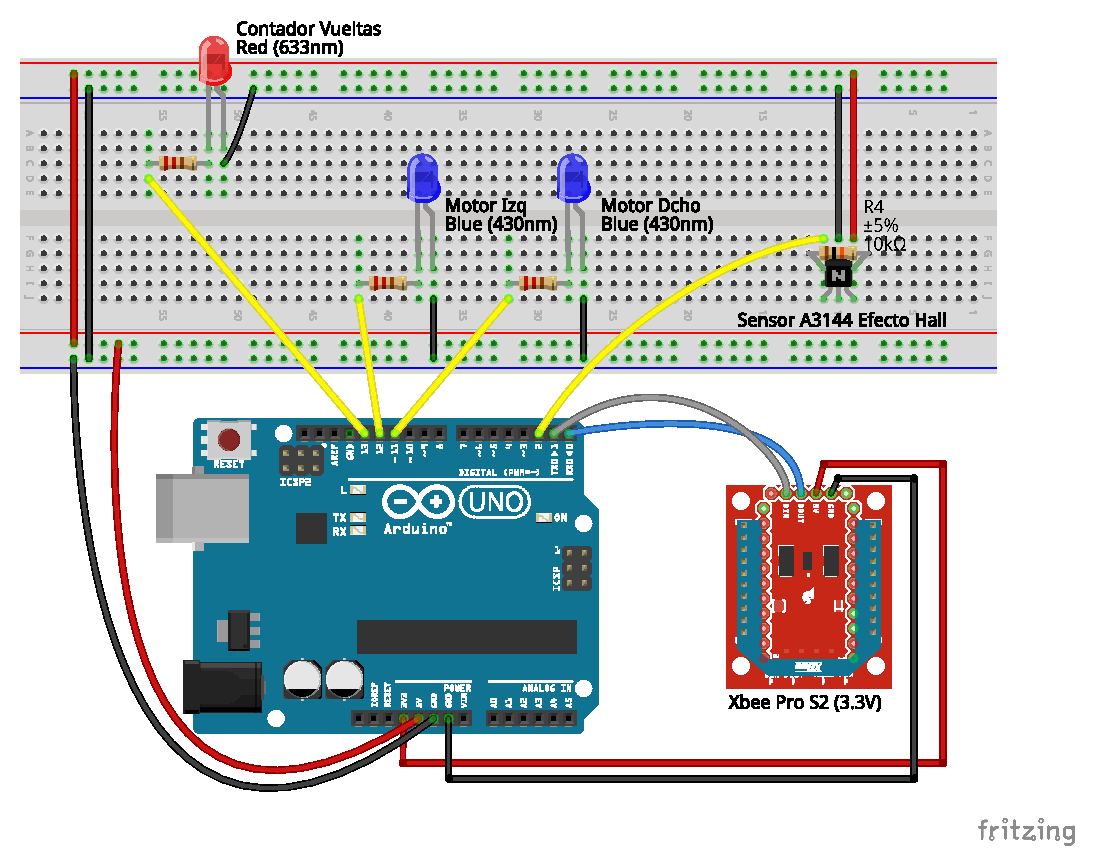
\includegraphics[width=.92\textwidth]{./figures/ProtocoloLEDS.pdf}
	\label{fig:ProtocoloLEDS}
	\caption{Maqueta de pruebas del protocolo de comunicación}
\end{figure}

Los dos leds de color azul representan los motores del vehículo. El led rojo representa el contador de las vueltas completas que realizan las ruedas de los motores. Y el sensor A3144 representa el sensor que está instalado en la rueda para contar cada vuelta que realizan. El vehiculo posee dos sensores de efecto Hall, uno para cada rueda, y cada rueda llevará un imad de neodimio para activar el sensor y, de esta manera, contar las vuelatas realizadas.


Para monitorizar el conteo de vueltas se utiliza el led de color rojo. Este se apaga cada vez que se aproxima el imán al sensor de tal forma que nos permite observar a simple vista si el contador se incrementa.

Los dos leds de color azul emulan la activación de los dos motores del vehículo. Uno representa el motor izquierdo y otro el derecho. Estos leds nos sirven para saber en que dirección se va a mover el vehículo. Ya que por ejemplo si se encienden los dos leds, significa que se está realizando un movimiento hacia delante. Solo se encienden los leds cuando se activan los motores por lo que nos permite saber si ha recibido la información cuando se enciende alguno de los dos leds. Y también permite saber cuando se ha terminado una orden si están los dos leds apagados.

 \section{Desarrollo del firmware para el control del vehículo}\label{sec:ConfiguracionCoche}
La programación del vehículo realizará en el lenguaje \emph{Arduino}. Dado que se utiliza un protocolo específico para este proyecto es necesario implementar una estructura para extraer la información de los paquetes de información en variables que el sistema pueda manejar. Como se explicó en la sección anterior la información viene estructurada en tres bloques. En primer lugar se comprueba si la información correspondiente al primer byte (ID) es igual al paquete de información que se espera. Es decir, si el movimiento que el vehículo espera, cronológicamente, es el primero, el identificador debe ser igual a 0. De no ser así el sistema no tratará la información de ese paquete ya que la información no corresponde al movimiento esperado. Una vez el identificador corresponde al paquete de información esperado se extrae la información del segundo byte correspondiente a la acción que se quiere realizar. Recordar que el segundo byte de información posee datos de la acción que se quiere realizar y del número de movimientos. Por ello se debe aplicar una máscara para extraer los tres bits mas significativos correspondientes a la acción de  movimiento. 

Si extraemos la información de esta forma se puede proceder a realizar los movimientos correspondientes al paquete de información recibido.

Luego se procederá a activar los motores y con ellos el contador correspondiente al número de vueltas que realizan las ruedas. Cuando el contador alcance el número de vueltas correspondientes al paquete de información, el programa devolverá un \ac{ACK} correspondiente a la realización de la orden. Si por algún problema el vehículo no logra realizar los movimientos esperados, el timeout se cumplirá y se comunicará a la placa \emph{Zedboard} que el movimiento no ha sido realizado correctamente. El sistema lanzará de nuevo el proceso principal para que calcule una nueva trayectoria correspondiente al estado actual del escenario. De no ser así el vehículo podría haber realizado un número de vueltas inferior al esperado y estar colocado en un lugar distinto del que el sistema tiene calculado en su trayectoria, por lo que la información se quedaría desfasada y no correspondería a la situación del momento.

Como la función \emph{loop} se ejecuta en bucle, el vehículo irá realizando movimientos a medida que las órdenes vayan siendo recibidas. Con la comprobación del identificador se controla que la orden es la que se espera y el coordinador de la placa \emph{Zedboard} será el encargado de ir enviando las órdenes en función de que se vayan cumpliendo. De esta forma, cuando el vehículo complete la trayectoria no recibirá más órdenes. A no ser que se proponga otro objetivo.

\section{Integración de los algoritmos en el sistema}\label{sec:Integracion}

Este proyecto está formado por una serie de algoritmos que en su conjunto forman el sistema. Antes de la integración de todos los algoritmos se ha realizado la implementación de cada uno de ellos de forma independiente. De acuerdo a la metodología ágil que se ha seguido se he intentado modularizar el proyecto por objetivos. Cada objetivo ha sido desarrollado hasta que se han conseguido los resultados esperados. De esta forma nos permite asegurar que, antes de la integración en el sistema, cada uno de estos algoritmos funciona de forma correcta. Este hecho evita muchos dolores de cabeza a la hora de afrontar los errores que se dan lugar en la fase de desarrollo.

Para poder integrar todos los algoritmos se ha decidido realizar una planificación acerca de cómo deben estar estructurados los datos de entrada y los resultados de cada algoritmo. A continuación se va a proceder a explicar cómo están organizados en función de los objetivos del sistema.

\begin{enumerate}
\item Distinción del vehículo sobre los demás objetos. Como argumento de entrada de este algoritmo se utilizará una imagen en formato \acx{JPG}\footnote{JPG es un formato de compresión de imágenes, tanto en color como en escala de grises, con alta calidad} en la cual aparezca el coche en el entorno, listo para calcular la trayectoria desde la ubicación en la que se encuentra. Los resultados de este algoritmo generarán un fichero de texto en el cual se guardará la información correspondiente a la coordenada en la que se encuentra el coche. 
\item Detección de obstáculos. Para poder detectar los obstáculos es necesario que se utilicen dos imágenes como argumentos del algoritmo. Estas imágenes están en formato \ac{JPG}, pero el algoritmo está implementado de tal forma para que se puedan utilizar distintos tipos. Como por ejemplo, \ac{BMP}, \acx{TIFF}\footnote{Formato de archivo de imagenes etiquetada. Un formato de imagen de alta resolución basado en etiquetas. TIFF se utiliza para el intercambio universal de imágenes digitales.}, \acx{PNG}\footnote{PNG (Portable Network Graphics) es un formato gráfico basado en un algoritmo de compresión sin pérdida para bitmaps no sujeto a patentes.}... Los resultados obtenidos serán reflejados en un fichero de texto, cuya extensión es .txt, y mediante el cual se reflejará el mapa binario en el que los obstáculos se representan con 1 y el camino libre con 0. 
\item Cálculo de trayectoria. Este algoritmo utilizará los datos contenidos en dos ficheros de texto. Uno de ellos corresponderá al mapa binario que se dio resultado en la ejecución del algoritmo de detección de obstáculos, mientras que el otro fichero guardará la información correspondiente a la coordenada de origen en la que se encuentra el vehículo. Como resultado de la aplicación del algoritmo se generará un fichero de texto en el cual se integre en el mapa la representación de la trayectoria que debe realizar el vehículo desde el punto de origen al destino. Esta trayectoria se representará mediante el número 3 para reflejar el comienzo, el número 2 para reflejar la ruta y el número 4 para el destino. De esta forma el mapa representará la ruta y los obstáculos contenidos en el entorno. Por otra parte se generará un fichero de texto en el cual se almacenarán todas las coordenadas correspondientes a todos los puntos que ha recorrido la trayectoria desde el inicio hasta su fin. Además, como forma de monitorización de los resultados también se generará una imagen en formato \ac{JPG} en la cual se distinga el mapa y la trayectoria mencionadas anteriormente. 
\item Generación de movimientos mediante datos de la trayectoria. Para la ejecución de este algoritmo es necesario un fichero de texto en el cual se representen todos los movimientos desde el inicio hasta el final de la trayectoria. Como resultado, el algoritmo no generará ningún fichero como tal pero establecerá la comunicación con el coche para que vaya ejecutando los movimientos correspondientes a la trayectoria.
\item Movimiento del vehículo. Para la ejecución de este algoritmo es necesario que se establezca una comunicación entre la placa \emph{Zedboard} y \emph{Arduino}. De tal forma que la información que reciba el coche sea interpretada para realizar los movimientos correspondientes a la orden.
\end{enumerate}

Teniendo en cuenta los argumentos y resultados recientemente enumerados, se debe realizar una implementación general del sistema en la que se incluyan todos los algoritmos de forma modular. Es decir, que exista una única función \textit{main} desde la cual se llame a las funciones que realizan los objetivos del sistema. De esta forma si en la ejecución ocurre algún error es fácil comprobar en que llamada ha ocurrido ya que aparecerá el nombre de la función en cuestión y será sencillo comprobar que ocurre. Además, de esta forma el proyecto se encuentra organizado por funcionalidades lo cual permite ejecutar los algoritmos del sistema que se deseen sin necesidad de comentar o eliminar el código que no se quiera utilizar.

Una vez conseguido el objetivo de la integración, se realizó una medición de los tiempos de ejecución del sistema y se comprobó que todos los algoritmos tienen un tiempo de ejecución menor a un segundo excepto el algoritmo de cálculo de trayectoria. Se podría considerar el cuello de botella del sistema. En el cuadro \ref{tab:TiemposEjecucionSoftware} se pueden observar algunos de los tiempos de ejecución calculados:

\begin{table}[hbtp]
  \centering
  \begin{tabular}{|c|c|c|c|c|c|c|c|c|}
    \hline
   \multicolumn{1}{|c|}{} & \multicolumn{2}{c|}{Coordenadas} & \multicolumn{2}{c|}{Tiempos Ejecución} \\ \cline{2-5}
    \multicolumn{1}{|c|}{}&Inicio&Final&4 direcciones& 8 direcciones\\
    \hline
    Diagonal&(0,0)&(1919,1079)&4.27 \textbf{min} &0.38 seg \\
    \hline
    Diagonal&(0,1079)&(1919,0)&31.15 \textbf{min}&0.40 seg\\
    \hline
    Centro&(959,539)&(961,541)&0.28 seg&0.37 seg\\
    \hline
    Centro&(959,541)&(961,539)&0.29 seg&0.34 seg\\
    \hline
    Abajo Arriba&(959,0)&(961,1079)&9.62 seg&3.20 seg\\
    \hline
    Arriba Abajo&(961,1079)&(959,0)&2.102 seg&2.57 \textbf{min}\\
    \hline
    Izq Dcha&(0,539)&(1919,541)&0.37 seg&1.60 seg\\
    \hline
    Dcha Izq&(1919,541)&(0,539)&0.34 seg&0.37 seg\\
    \hline
  \end{tabular}
  \caption{Tiempos de ejecución en software}
  \label{tab:TiemposEjecucionSoftware}
\end{table}

Como se puede observar en algunos casos el tiempo de ejecución es bastante mayor a un segundo. Se aumenta el orden de magnitud a minutos en un par de casos. Aunque en el sistema final solo se calcula la trayectoria para 8 direcciones, hay un caso en el que tarda alrededor de 3 minutos para calcular la trayectoria. Es por ello que se decidió realizar una optimización desarrollando un nuevo código que mediante el uso de hardware reconfigurable se obtienen tiempos de ejecución mejores.

Dado que el único algoritmo que suponía una limitación en cuanto al tiempo de ejecución fue el algoritmo A*, el resto se decidió que puede ejecutarse en el procesador \ac{ARM} de la placa \emph{Zedboard} utilizándose las librerías de \emph{OpenCV} para un par de casos en los cuales se podría realizar una optimización. Cabe mencionar que el objetivo de este \ac{TFG} se pudo realizar con la integración de los algoritmos que hemos visto hasta ahora sin optimizar. A continuación se va a proceder a desarrollar las optimizaciones que se han llevado a cabo en el sistema. 

\section{Optimizaciones realizadas en el sistema}\label{sec:Optimizaciones}

\subsection{Dilatación de obstáculos mediante \emph{OpenCV}}\label{sec:DilatacionObjetos}

Tras asistir a una charla acerca de procesamiento de imágenes que se propuso en el laboratorio ARCO, se planteo modificar el algoritmo de detección de objetos ya que la implementación de la delimitación de obstáculos es compleja. Uno de los temas que se abordó en la charla fueron los algoritmos de erosión y dilatación para el tratamiento de información de una imagen. En el momento, la charla no iba orientada a este \ac{TFG}, sino que se mostraron ejemplos de cómo procesar la información de fotografías y ver cómo afectaban distintos tipos de operaciones en el resultado. Pero tras mencionar cómo funcionaban los algoritmos de erosión y dilatación se vislumbró la idea de adaptarlo al sistema.

Una de las razones por las que se delimitan los obstáculos del entorno en cuadrados o rectángulos es para evitar que el vehículo colisione debido a la irregularidad de los obstáculos. Es decir, que debido a su forma irregular el vehículo colisione con los objetos. Otra de las razones, si la distancia entre un objeto u otro es menor que las medidas del vehículo, el algoritmo de cálculo de trayectoria puede encontrar un ruta que en principio es óptima pero que ocasionaría una colisión debido a que el vehículo no cabe entre ambos objetos. ¿Qué ocurriría si se decide dilatar el grosor de los obstáculos en función de las medidas del vehículo? 

\begin{figure}[hbtp]
 \centering
  \subfloat[Imagen sin objetos]{
    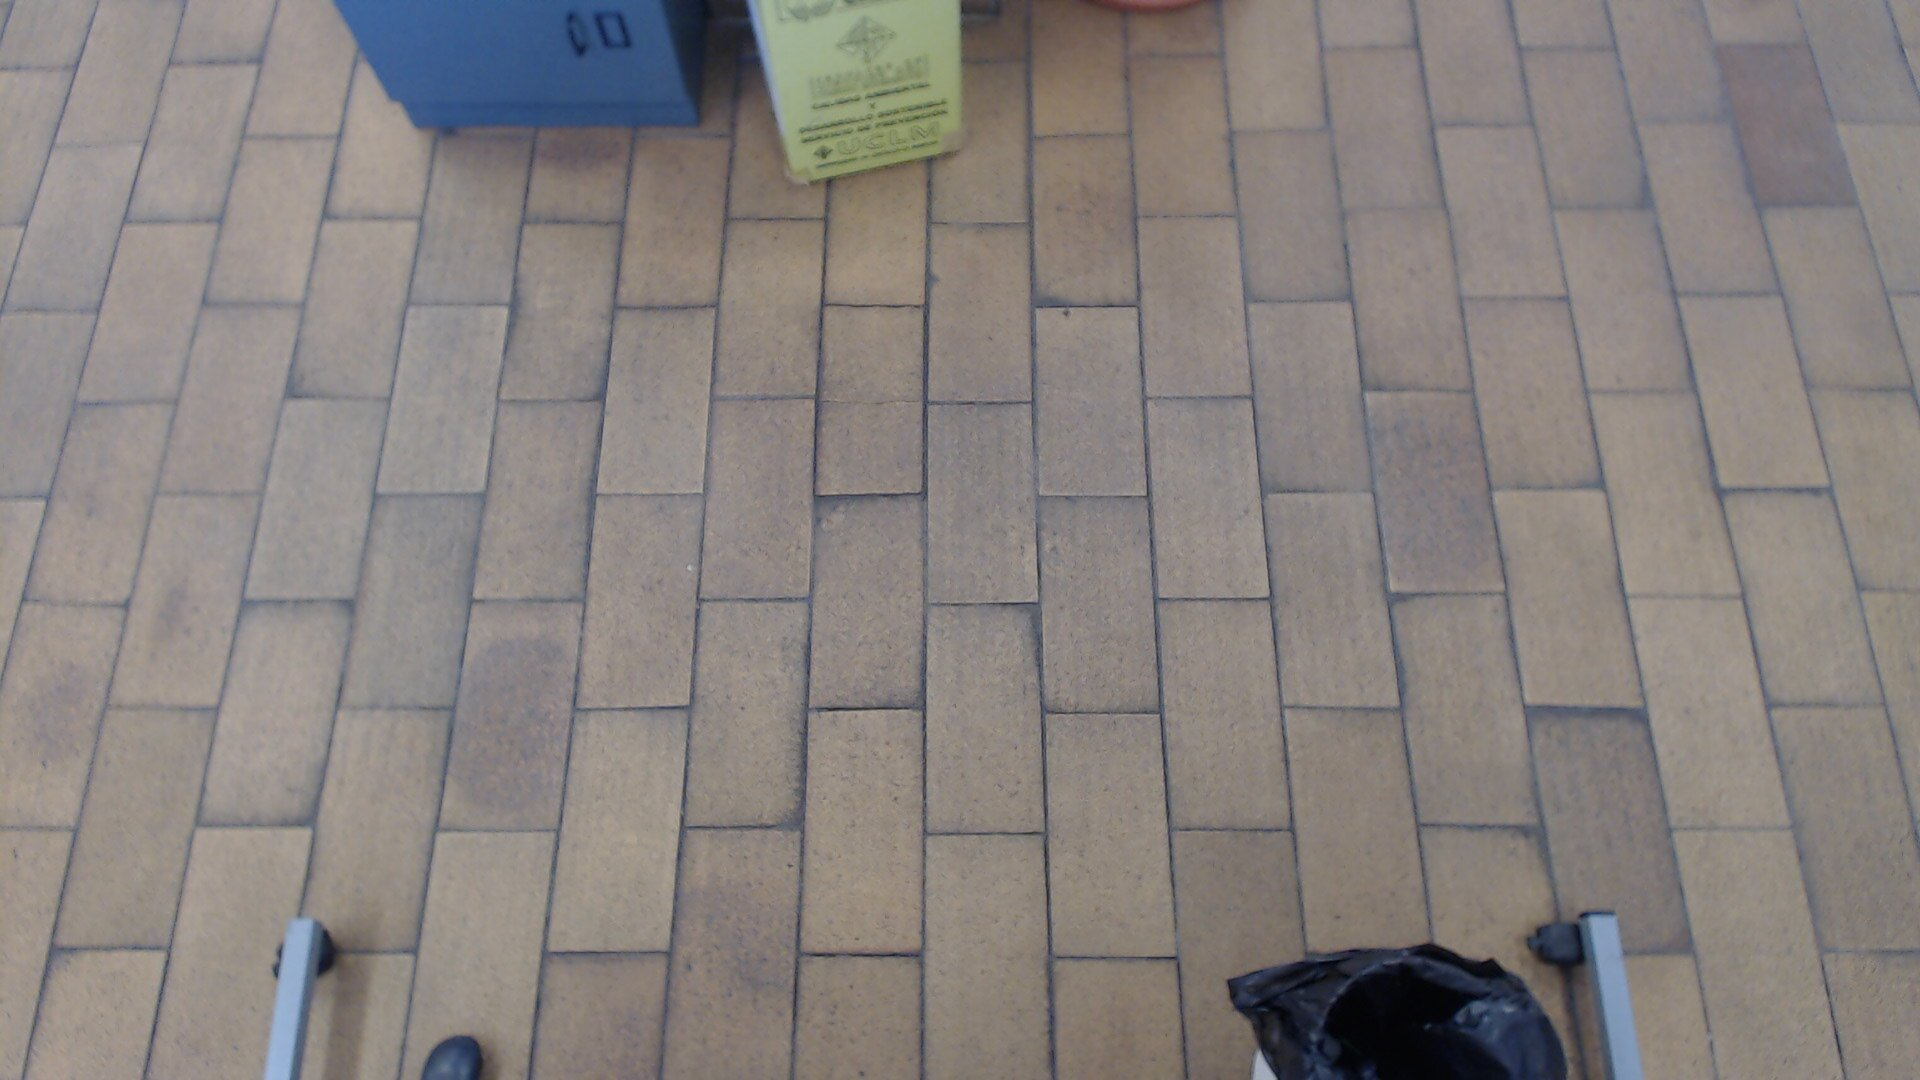
\includegraphics[width=0.33\textwidth]{./figures/EscenarioDilatacion.jpeg}}
  \subfloat[Imagen con objetos]{
    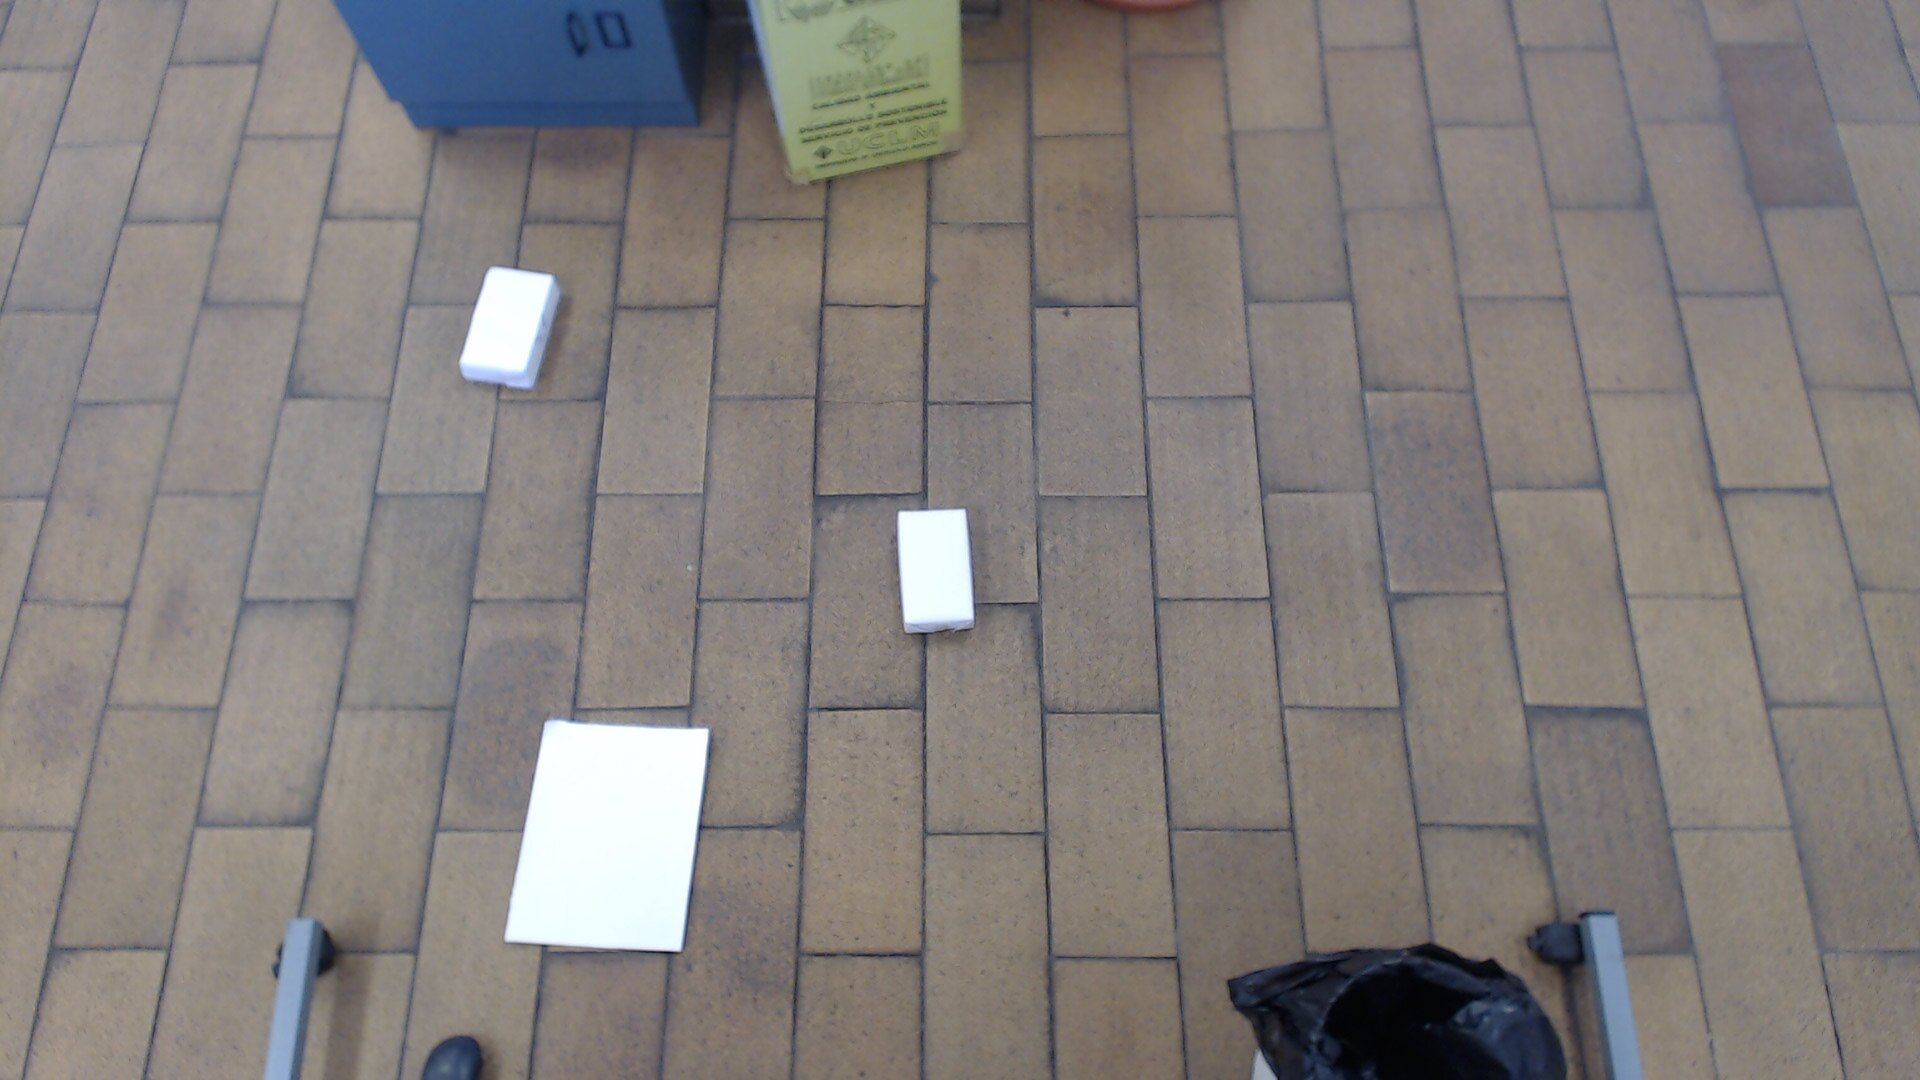
\includegraphics[width=0.33\textwidth]{./figures/ObjetosDilatacion.jpg}}
  \subfloat[Imagen Dilatada]{
    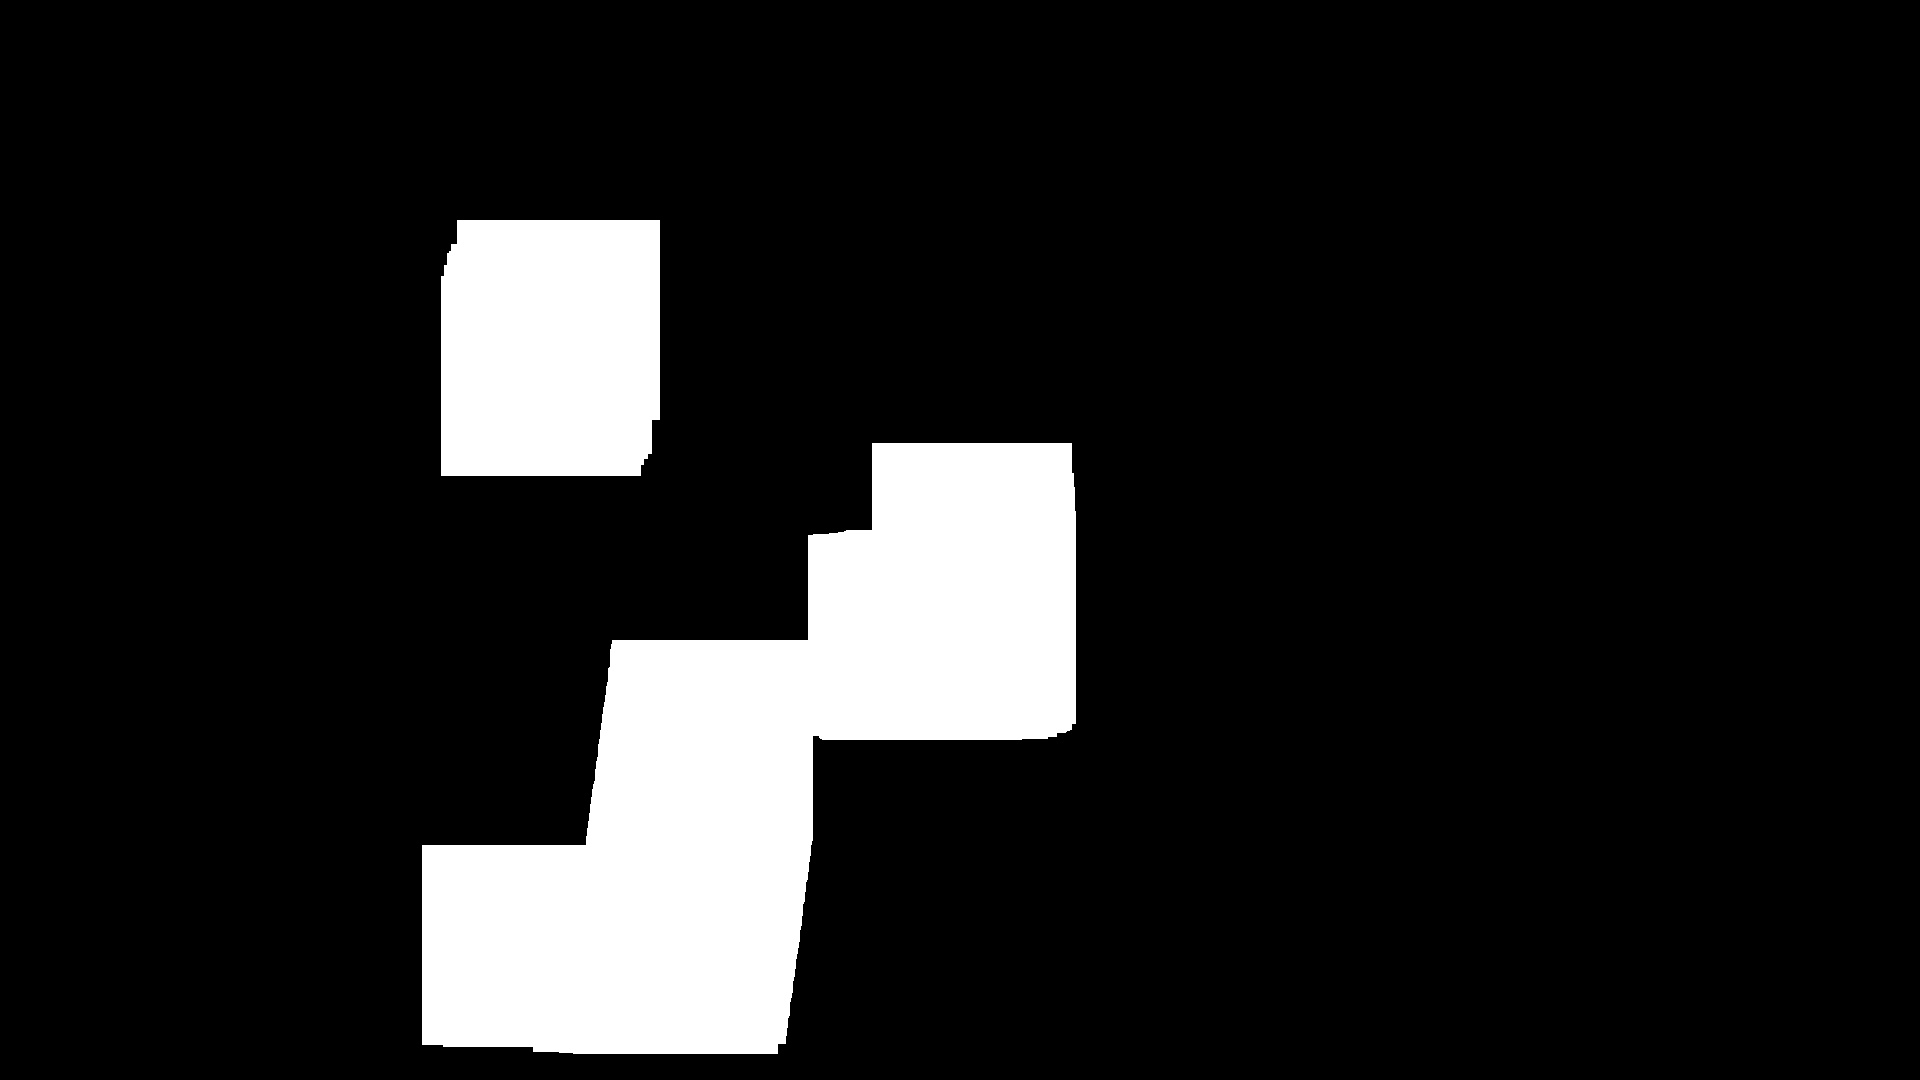
\includegraphics[width=0.33\textwidth]{./figures/objetosDilatados.jpeg}}
 \caption{Ejemplo de dilatación de objetos}
 \label{fig:dilatacion}
\end{figure}

La operación de dilatación consiste en aplicar una máscara que modifique los valores que se encuentran alrededor del píxel objetivo. De tal manera que expanda el valor del píxel en función del tamaño que se le introduzca como argumento. Un ejemplo de dilatación sería el de la figura \ref{fig:dilatacion}. La librería \emph{OpenCV} posee un método que aplica la dilatación en función de un tamaño como parámetro. Si en dicho argumento se introduce el tamaño del vehículo, este algoritmo dilatará el valor de los objetos, es decir el valor 1, alrededor del píxel origen hasta que se corresponda con el tamaño del vehículo en todos su píxeles vecinos. De esta forma mediante la utilización de la librería se puede evitar utilizar el algoritmo implementado anteriormente ya que la complejidad del proceso origina un peor rendimiento en comparación con la función de dilatación optimizada de \emph{OpenCV}. 

\subsection{Tratamiento de la información de una imagen en varios formatos}\label{sec:ImagenesJPG}

Debido a que en un primer lugar la idea era embeber\footnote{Un sistema embebido o empotrado (integrado, incrustado) es un sistema de computación diseñado para realizar una o algunas pocas funciones dedicadas, frecuentemente en un sistema de computación en tiempo real.} todo el sistema en la placa \emph{Zedboard}, se evitó utilizar la librería de OpenCV para el tratamiento de los datos de una imagen. Ya que, como se introdujo en el capítulo de objetivos \ref{chap:objetivos}, el uso de las herramientas de \emph{Vivado} poseen una serie de restricciones en los mecanismos de programación y el uso de librerías está limitado al soporte de la propia herramienta. Por ejemplo la librería de OpenCV ofrece muchas más funciones de las que la herramienta Vivado HLS da soporte \cite{RestriccionesOpenCV}. Como consecuencia de evitar utilizar \emph{OpenCV}, se decidío implementar un programa para extraer la información de imágenes en formato \ac{BMP}\footnote{BMP es un formato de imagen de mapa de bits, propio del sistema operativo Microsoft Windows.}. Posteriormente se realizó otra implementación, pero esta vez utilizando la librería \emph{OpenCV}. 

La librería \emph{OpenCV} nos proporciona el objeto tipo \emph{Mat} que es de gran utilidad a la hora de trabajar con imágenes. Ya que nos permite interactuar con  una gran cantidad de funciones con las que podemos realizar infinidad de operaciones. \cite{Mat} En este proyecto, para el tratamiento de la información de una imagen, se ha utilizado la función \emph{imread}. \cite{ImRead}

Con el uso de esta función solo tenemos que preocuparnos de introducir la ruta en la que se encuentra la imagen como primer argumento. Y como segundo argumento cualquiera de estas tres opciones:

\begin{enumerate}
\item CV\_LOAD\_IMAGE\_UNCHANGED. Si se quiere cargar el valor alpha, normalmente hace referencia a la intensidad, en el objeto \emph{Mat}. Es decir, cuatro bytes de información por píxel. Uno para el canal alpha y tres para el modelo de color \ac{RGB}.
\item CV\_LOAD\_IMAGE\_GRAYSCALE. Si se quiere guardar la información de la imagen en formato de escala de grises. Es decir, un byte de información por píxel.
\item CV\_LOAD\_IMAGE\_COLOR. Si se quiere guardar la imagen en modelo de color \ac{RGB}. Es decir, tres bytes por píxel.
\end{enumerate}

Con esta función, con una simple línea de código se interpreta la información de la cabecera, los datos en crudo de la imagen y hasta se puede cambiar el número de canales que posee la imagen en la misma llamada. Para la detección de objetos el algoritmo utiliza como argumentos las imágenes en escala de grises con formato \acx{JPG}, que es el formato de salida por defecto de la cámara cenital que se utiliza en el proyecto. Por lo que no es necesario realizar ningún tipo de conversión. Además, la función \emph{imread} permite utilizar los formatos \ac{BMP}, \acx{JPEG}, \ac{TIFF}, \ac{PNG} y algunos más que no son necesarios mencionar. \cite{ImRead}

\subsection{Segmentación de la imagen en macro-bloques}\label{subsec:macrobloques}

Como consecuencia de la utilización de imágenes \emph{FullHD}, el mapa utilizado en el algoritmo de cálculo de trayectoria es grande, ya que la cantidad de nodos por los que se puede recorrer la trayectoria del vehículo es superior a 2 millones. Esto implica que los tiempos de ejecución del algoritmo A* se disparen en función del escenario en el que se encuentren. Bien tardando segundos o minutos en calcular la trayectoria. Es por ello que se ha decidido segmentar la información del mapa en macro-bloques que guarden la información relevante de la imagen, en este caso los obstáculos. 

\begin{figure}[hbtp]
\centering
	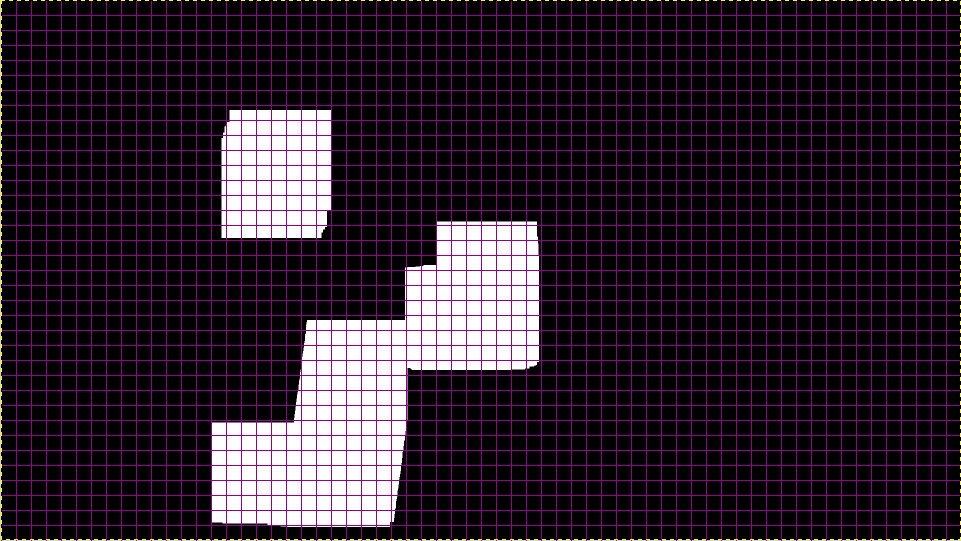
\includegraphics[width=.9\textwidth]{./figures/rejilla.jpeg}
	\label{fig:rejilla}
	\caption{Ejemplo de segmentación de imagen en macro-bloques}
\end{figure}

La división del escenario en bloques permite que se pueda re-escalar la imagen a una resolución menor. Ahora bien, cada píxel de la nueva imagen contiene la información de interés de la sección a la que corresponde en el escenario. Esta información hace referencia a la cantidad de obstáculos que se encuentran en dicha sección. Como tras la aplicación del algoritmo de dilatación se genera un mapa binario en el que un 1 corresponde a un obstáculo y un 0 corresponde a una posición por la que el vehículo puede pasar, se decidió realizar una sumatoria de todos los valores que se encuentran en el bloque para saber si una sección está llena de obstáculos o por el contrario vacía. Al utilizar una resolución \emph{FullHD} se ha buscado una resolución menor con la que se pueda guardar la proporción de la imagen. Esta resolución es 64x36, ya que no genera ningún valor flotante con el que podríamos perder información. Con dicha resolución, pasamos de tener más de 2 millones de píxeles a 2048 píxeles por imagen, cada bloque tiene un tamaño de 30x30 píxeles. Si la sección correspondiente al mapa tiene un valor equivalente a 900 significa que este bloque está completamente ocupado por un obstáculo. Mientras que si por el contrario tiene un valor 0 está completamente libre de obstáculos. Se puede dar el caso intermedio en el que el valor de dicho bloque se encuentre entre 900 y 0. Cuanto más se acerque a 900 más completo estará de obstáculos mientras que cuanto más bajo sea menos obstáculos se encontrarán en el bloque. Esto genera un inconveniente, ya que aunque el valor del bloque sea 30 puede ser que el obstáculo que aparece en la sección bloquee el camino de ese nodo. Es por ello, que para evitar posibles problemas se ha decidido que si el valor de un bloque es mayor que 0 se asigne un 1. De esta forma la ruta calculada no es óptima en cuanto a distancia, pero se reduce mucho el tiempo de ejecución del algoritmo de cálculo de trayectoria ya que hemos pasado de manejar más de 2 millones de nodos a 2048 nodos para el peor caso de pruebas.

De esta forma se ha reducido el tamaño del mapa que se pasa al algoritmo de cálculo de trayectoria. Esto implica que los tiempos de ejecución mejoren mucho ya que el número de recursos que utiliza es mucho menor. La ruta que genera no es óptima en cuanto a la distancia pero es muy similar a la que se calcula en la resolución \emph{FullHD}.

\subsection{Implementación algoritmo A* según restricciones de \emph{Vivado HLS}}\label{sec:HLSCalculoTrayectoria}

Una vez llegados a este punto se decidió embeber en hardware reconfigurable el algoritmo de cálculo de trayectoria con la intención de optimizar el tiempo de ejecución. 
Para ello se hará uso de la herramienta \emph{Vivado} \ac{HLS}, mediante la cual generaremos un componente \ac{IP} con la funcionalidad del algoritmo para ser implementado en la FPGA.

Para poder crear este componente es necesario tener en cuenta la restricción principal de la herramienta \emph{Vivado} \ac{HLS}.

\begin{description}
\item [Restricción] No se puede utilizar asignación dinámica de memoria. 
\end{description}

Como consecuencia de esta limitación ha sido necesario implementar desde cero el algoritmo de cálculo de trayectoria ya que en un principio, como se dijo en la sección \ref{sec:AEstrellaSoftware}, se utilizó una modificación de una implementación del algoritmo A* que se encontró en internet. \cite{ImplementacionAlgoritmoA}

Los algoritmos de cálculo de trayectoria utilizan por defecto asignación dinámica de memoria para crear y destruir los nodos en función de la búsqueda. Es decir, cada vez que se comprueba algún nodo adyacente se reserva memoria para la información del nodo. Mientras que si por el contrario el nodo que se ha visitado no es necesario mantenerlo en memoria se elimina. Este tipo de operaciones no se pueden realizar ya que al embeber el algoritmo en hardware la placa no puede gestionar dinámicamente la memoria. Para ejecutar el algoritmo es obligatorio definir previamente que memoria debe reservar el sistema. Por ello, como primer paso para desarrollar la nueva implementación del algoritmo se decidió definir una estructura de datos con la cual se pueda acotar la  cantidad máxima de memoria necesaria para la resolución del peor caso posible.

\begin{table}[]
\centering
\begin{tabular}{|c|c|}
\hline
\multicolumn{2}{|c|}{\cellcolor[HTML]{9B9B9B}Estructura de datos tipo Nodos} \\ \hline
\rowcolor[HTML]{C0C0C0}
Variables & \multicolumn{1}{c|}{\cellcolor[HTML]{C0C0C0}Bits} \\ \hline
Coordenada X & 6 \\ \hline 
Coordenada Y & 6 \\ \hline
Posición del padre & 12 \\ \hline
Coste &  14     \\ \hline
Heurística & 7 \\ \hline
F (Coste + Heurística) & 21 \\ \hline
Visitado   & 1 \\ \hline
\end{tabular}
\caption{Estructura de datos de cada nodo del mapa.}
\label{tab:EstructuraNodos}
\end{table}

Según el cuadro \ref{tab:EstructuraNodos} cada nodo va a poseer una estructura de datos tipo Nodos. Este tipo de estructura nos permite definir una plantilla sobre la cual reservar la estructura de memoria necesaria para cada nodo del mapa. Gracias a esta definición se puede generar un vector unidimensional de nodos. Cada celda de este vector está representada por la estructura de datos tipo Nodos, sobre la cual se irá añadiendo la información correspondiente a los elementos del mapa. De esta forma podemos reservar la memoria de forma estática previamente a la ejecución del algoritmo y posteriormente, en tiempo de ejecución, ir actualizando las variables en función de la posición en la que se encuentre el nodo. Ahora bien, para poder ir actualizando los valores de la estructura tipo Nodos es necesaria la implementación de una función con la que calcular la posición de los nodos adyacentes a la posición inicial, de tal manera que cada vez que el algoritmo A* seleccione un nodo por el cual avanzar se calculen los nodos adyacentes al nodo actual.

Para calcular la posición unidimensional de los nodos adyacentes al nodo actual es necesario tener en cuenta una serie de premisas. Por ejemplo, hay que tener en cuenta los bordes del mapa. Es decir, según la posición en la que se encuentre el nodo actual no se pueden expandir todos los nodos adyacentes ya que puede ser que se encuentren fuera del mapa. Si nos encontramos en la posición unidimensional 0, la cual hace referencia a la esquina superior izquierda, hay una serie de nodos que no podemos expandir. Estos nodos serían los que hicieran referencia a los movimientos arriba, izquierda, diagonal superior izquierda, diagonal superior derecha y diagonal inferior izquierda. Existen más restricciones como esta, por ejemplo las esquinas restantes y si el nodo actual se encuentra en cualquier límite del mapa. Cada una de estas situaciones afecta a una posición adyacente distinta por lo que se ha decidido separar los nodos adyacentes por coordenada \emph{x} e \emph{y}. De esta forma primero se calcula la posición unidimensional correspondiente a la coordenada \emph{x} e \emph{y} que se pasa como argumento al método para posteriormente invalidar el valor de la posición si esta no puede expandirse debido a los límites del mapa. A continuación veamos un ejemplo de cómo se calculan los nodos adyacentes a la posición $x=0$, véase el listado de código \ref{code:NodosAdyacentes}

\begin{listing}[
  float=ht,
  language = C++,
  caption  = {Parte del algoritmo que calcula los nodos adyacentes},
  label    = code:NodosAdyacentes]
void adjacentNodes(int x, int y){
	int initPosition = x+(y*HORIZONTAL);
	//Left
	adjacentPosition[0][2] = initPosition-1; //Position
	//Right
	adjacentPosition[1][2] = initPosition+1; //Position
	//Top
	adjacentPosition[2][2]= initPosition-HORIZONTAL; //Position
	//Bot
	adjacentPosition[3][2] = initPosition+HORIZONTAL; //Position
	//Upper Left Diagonal
	adjacentPosition[4][2]= initPosition-HORIZONTAL-1; //Position
	//Upper Right Diagonal
	adjacentPosition[5][2] = initPosition-HORIZONTAL+1; //Position
	//Bottom Left Diagonal
	adjacentPosition[6][2] = initPosition+HORIZONTAL-1; //Position
	//Bottom Right Diagonal
	adjacentPosition[7][2] = initPosition+HORIZONTAL+1; //Position

	//if nodes are not adjacent set -1 on position.
	if(x==0){
		//Left
		adjacentPosition[0][2] = -1; //NotAdjacent
		//Right
		adjacentPosition[1][0] = x+1; //X
		//Top
		adjacentPosition[2][0] = x; //X
		//Bot
		adjacentPosition[3][0] = x; //X
		//Upper Left Diagonal
		adjacentPosition[4][2]= -1; //Not adjacent
		//Upper Right Diagonal
		adjacentPosition[5][0] = x+1; //X
		//Bottom Left Diagonal
		adjacentPosition[6][2] = -1; //Not adjacent
		//Bottom Right Diagonal
		adjacentPosition[7][0] = x+1; //X
	}else if...
\end{listing}

Como se puede observar, para almacenar los datos correspondientes a los ocho nodos adyacentes al nodo actual se ha generado una matriz bidimensional en la que la posición de la primera dimensión corresponde al identificador de los ocho posibles nodos adyacentes.La posición de la siguiente dimensión hace referencia a la coordenada X, coordenada Y y posición unidimensional en el vector de estructuras tipo Nodos, cuadro \ref{tab:EstructuraNodos}. Una vez que sabemos como está estructurada la información de los nodos adyacentes se puede observar que al comienzo se calcula la posición equivalente a la coordenada X e Y en el vector unidimensional. Como hay ocho posibles nodos adyacentes se calcula la posición correspondiente a las ocho direcciones posibles. Izquierda, derecha, arriba, abajo, diagonal superior izquierda y derecha y diagonal inferior derecha e izquierda. Posteriormente se comprueba si el nodo actual se encuentra en alguno de los límites del mapa. En este caso solo aparece $x=0$ debido a la longitud del código, pero habría un caso para $x=HORIZONTAL-1$, para los valores intermedios entre $x=0$ y $x=HORIZONTAL-1$ y lo mismo para la coordenada y. Es decir, $y=0$, $y=VERTICAL-1$ y los valores intermedios. Para $x=0$ los nodos adyacentes que no se pueden expandir son los de la izquierda, diagonal superior izquierda y diagonal inferior izquierda. Ya que son las posición en los que se resta uno al valor de la x. Y como vale 0, no puede ser negativo. Para los valores que no se pueden expandir se actualiza el valor a $-1$, el cual nos va a servir para identificar si es un nodo que hay que evitar en el futuro.

Una vez conocemos los nodos adyacentes se puede proceder a aplicar el algoritmo A*. Los pasos que sigue el algoritmo son los siguientes:

\begin{enumerate}
\item Inicializamos el vector unidimensional de estructuras tipo Nodos.
\item Inicializamos el nodo inicial de búsqueda. Correspondiente a la coordenada en la que se encuentra el vehículo.
\item Calculamos los nodos adyacentes al nodo inicial.
\item Calculamos cúal es la posición del padre, que coste tiene avanzar a la posición adyacente y la heurística que evalúa la distancia entre la posición actual y el destino.
\item Calculamos la mejor opción de los nodos adyacentes.
\item Establecemos la mejor opción como visitada.
\item Inicializamos el bucle que realiza la búsqueda hasta que llega a la posición final.
\begin{enumerate}
\item Calculamos los nodos adyacentes al nodo actual.
\item Calculamos el padre, el coste y la heurística del movimiento.
\item Elegimos la mejor opción entre la lista de nodos abiertos. Incluye los nodos adyacentes y los nodos calculados previamente que no han sido visitados. Esta implementación de una lista de nodos abiertos es la que nos permite asegurar que el resultado obtenido es óptimo. Ya que va desarrollando la ruta en función del mejor valor, no del mejor adyacente.
\item Establecemos la mejor opción como visitada para evitar volver a pasar.
\end{enumerate} 
\item Una vez se ha calculado la ruta nos situamos en la posición final y vamos preguntando quién es el padre del nodo actual hasta que llegamos a la posición inicial. De esta forma se guarda la trayectoria que se ha seguido.
\end{enumerate}

Para la implementación de este algoritmo se han ido desarrollando las funciones en función de la lista de pasos comentada previamente. Como base teórica del algoritmo se ha seguido la explicación del algoritmo, sin implementación, de la página web \cite{APrincipiantes}. A continuación se va a proceder a explicar cómo se ha resuelto cada uno de estos pasos.

\subsubsection{Inicialización del vector unidimensional de estructuras tipo Nodos}\label{subsec:InitNodes}

Dado que el archivo sobre el cual obtenemos los datos del mapa viene representado de forma bidimensional se decidío implementar un algoritmo con el cual se pudiera inicializar la matriz unidimensional, de estructuras tipo Nodos, a través del archivo bidimensional. Para ello, se pensó en recorrer la matriz en función del tamaño, $horizontal*vertical$, de esta forma se recorre la misma distancia para el formato bidimensional y unidimensional. Se debe tener en cuenta que cada vez que se recorra el tamaño correspondiente al tamaño horizontal se debe incrementar el valor de la coordenada Y. De esta forma se recorrerá la matriz unidimensional y se podrán guardar los valores correspondientes a la coordenada X e Y del mapa. Los valores de la coordenada X e Y se utilizan para consultar en el mapa si en la coordenada correspondiente hay un obstáculo o es camino transitable. Si el camino es transitable se inicializa el valor de visitado a $0$, mientras que si es un obstáculo se inicializa a $1$. Así se evita calcular la información correspondiente al nodo. Como resultado obtenemos el vector unidimensional de estructuras tipo Nodos con las coordenadas X e Y correspondientes a su posición y la información acerca de si los nodos se pueden visitar o no.

\subsubsection{Inicialización del nodo inicial de búsqueda}\label{subsec:InitStart}

El nodo inicial de búsqueda es el correspondiente a las coordenadas iniciales en las que se encuentra el vehículo. Por lo que es necesario extraer la información del fichero que genera el algoritmo de detección del vehículo de la sección \ref{sec:DeteccionVehiculo}. Una vez se obtienen las coordenadas X e Y se calcula la posición unidimensional correspondiente, como aparece al comienzo del listado \ref{code:NodosAdyacentes}, y se inicializa a $1$ el campo correspondiente a visitado.

\subsubsection{Cálculo de los nodos adyacentes al nodo inicial}\label{subsec:NodosAdyacentesStart}

Se llama a la función \emph{adjacentNodes}, mencionada anteriormente en el listado \ref{code:NodosAdyacentes}, con las coordenadas X e Y en las que se encuentra el vehículo como argumentos.

\subsubsection{Actualizamos la información de los nodos adyacentes}\label{subsec:ActualizarNodosAdyacentes}

Para calcular y actualizar la información de los nodos se deben recorrer los 8 nodos adyacentes posibles. Una vez se comprueba si el nodo se puede visitar, bien porque no sea un obstáculo o porque no se encuentre en el límite del mapa, se procede a incluir el nodo en la lista de nodo abiertos. Posteriormente se actualiza la información del padre, que en este caso es el nodo en el que se encuentra el vehículo. Se calcula la heurística con la función de \emph{Manhattan}, la cual actualiza el valor según el código del listado \ref{code:Manhattan}. A continuación se calcula el coste al que equivaldría la ejecución del movimiento al nodo adyacente. Este coste es acumulativo, pero como estamos al principio se suman 10 si el movimiento es ortogonal y 14 si el movimiento es diagonal. Por último se suma el coste y la heurística y se guarda en la variable \emph{costPlusHeuristic}.

\begin{listing}[
  float=ht,
  language = C++,
  caption  = {Función con la que se calcula la heurística},
  label    = code:Manhattan]
void manhattanHeuristic(int x, int y, int position, int xFinish, int yFinish){
	int xDistance, yDistance;
	xDistance = xFinish - x;
	yDistance= yFinish - y;

	node[position].heuristic = abs(xDistance)+abs(yDistance);
}
\end{listing}

\subsubsection{Calculamos la mejor opción de los nodos adyacentes}\label{subsec:BestOption}

Una vez se ha actualizado la información de los 8 nodos adyacentes al nodo actual se realiza una comparación entre los valores de la variable \emph{costPlusHeuristic} de cada nodo que aparezca en la lista de nodos abiertos. Esta lista puede contener los nodos adyacentes y los nodos que se han calculado previamente. Como en este caso solo hemos calculado los nodos adyacentes del punto inicial, la lista de nodos abiertos estará formada solo por los adyacentes. Al comprobar si el nodo se encuentra en la lista abierta se evita contar con nodos que no son accesibles o ya están visitados. Si el valor de la variable \emph{costPlusHeuristic} es menor que el mejor valor guardado previamente se sustituye y se almacena la posición correspondiente al mejor nodo. De esta forma tras recorrer todos los nodos de la lista abierta se devuelve la posición correspondiente al mejor nodo por el que continuar la trayectoria. Véase el listado de código \ref{code:BestOption}.

\begin{listing}[
  float=ht,
  language = C++,
  caption  = {Función con la que se calcula el mejor nodo},
  label    = code:BestOption]
int calculateBestOption(){
	int bestOption = 2147483647;
	int positionBestOption;

	for (int i = 0; i < (HORIZONTAL*VERTICAL); i++) {
		if(openNodes[i]==0){ //If it is an open node
			if( node[i].costPlusHeuristic < bestOption ){ //If is a better option...
				bestOption = node[i].costPlusHeuristic;
				positionBestOption = i;
			}
		}
	}

	return positionBestOption;
}
\end{listing}

\subsubsection{Establecer la mejor opción como visitada}\label{subsec:NodoVisitado}

Una vez se ha calculado cual es la posición sobre la que debe avanzar el vehículo se actualiza la variable $visited=1$, De esta forma se evita volver a pasar por el mismo nodo en futuros movimientos.

\subsubsection{Inicialización del bucle para calcular la trayectoria}\label{subsec:BucleA}   

Los pasos mencionados anteriormente se han aplicado para inicializar la búsqueda, a continuación se debe establecer un bucle hasta que se cumpla la condición de que el nodo actual corresponda a la posición correspondiente al destino. 

El proceso que se lleva a cabo en el bucle es el mismo, existe una pequeña variación ya que la posición que se envía como argumento a los métodos es distinta en función del avance de la trayectoria. Por ello cada iteración del bucle genera unos nuevos nodos adyacentes a la posición actual que se añaden a la lista de nodos abiertos que debe valorar el algoritmo. 

\section{Integración del sistema en la placa \emph{Zedboard} }\label{sec:IntegracionZedboard}

\begin{figure}[hbtp]
\centering
	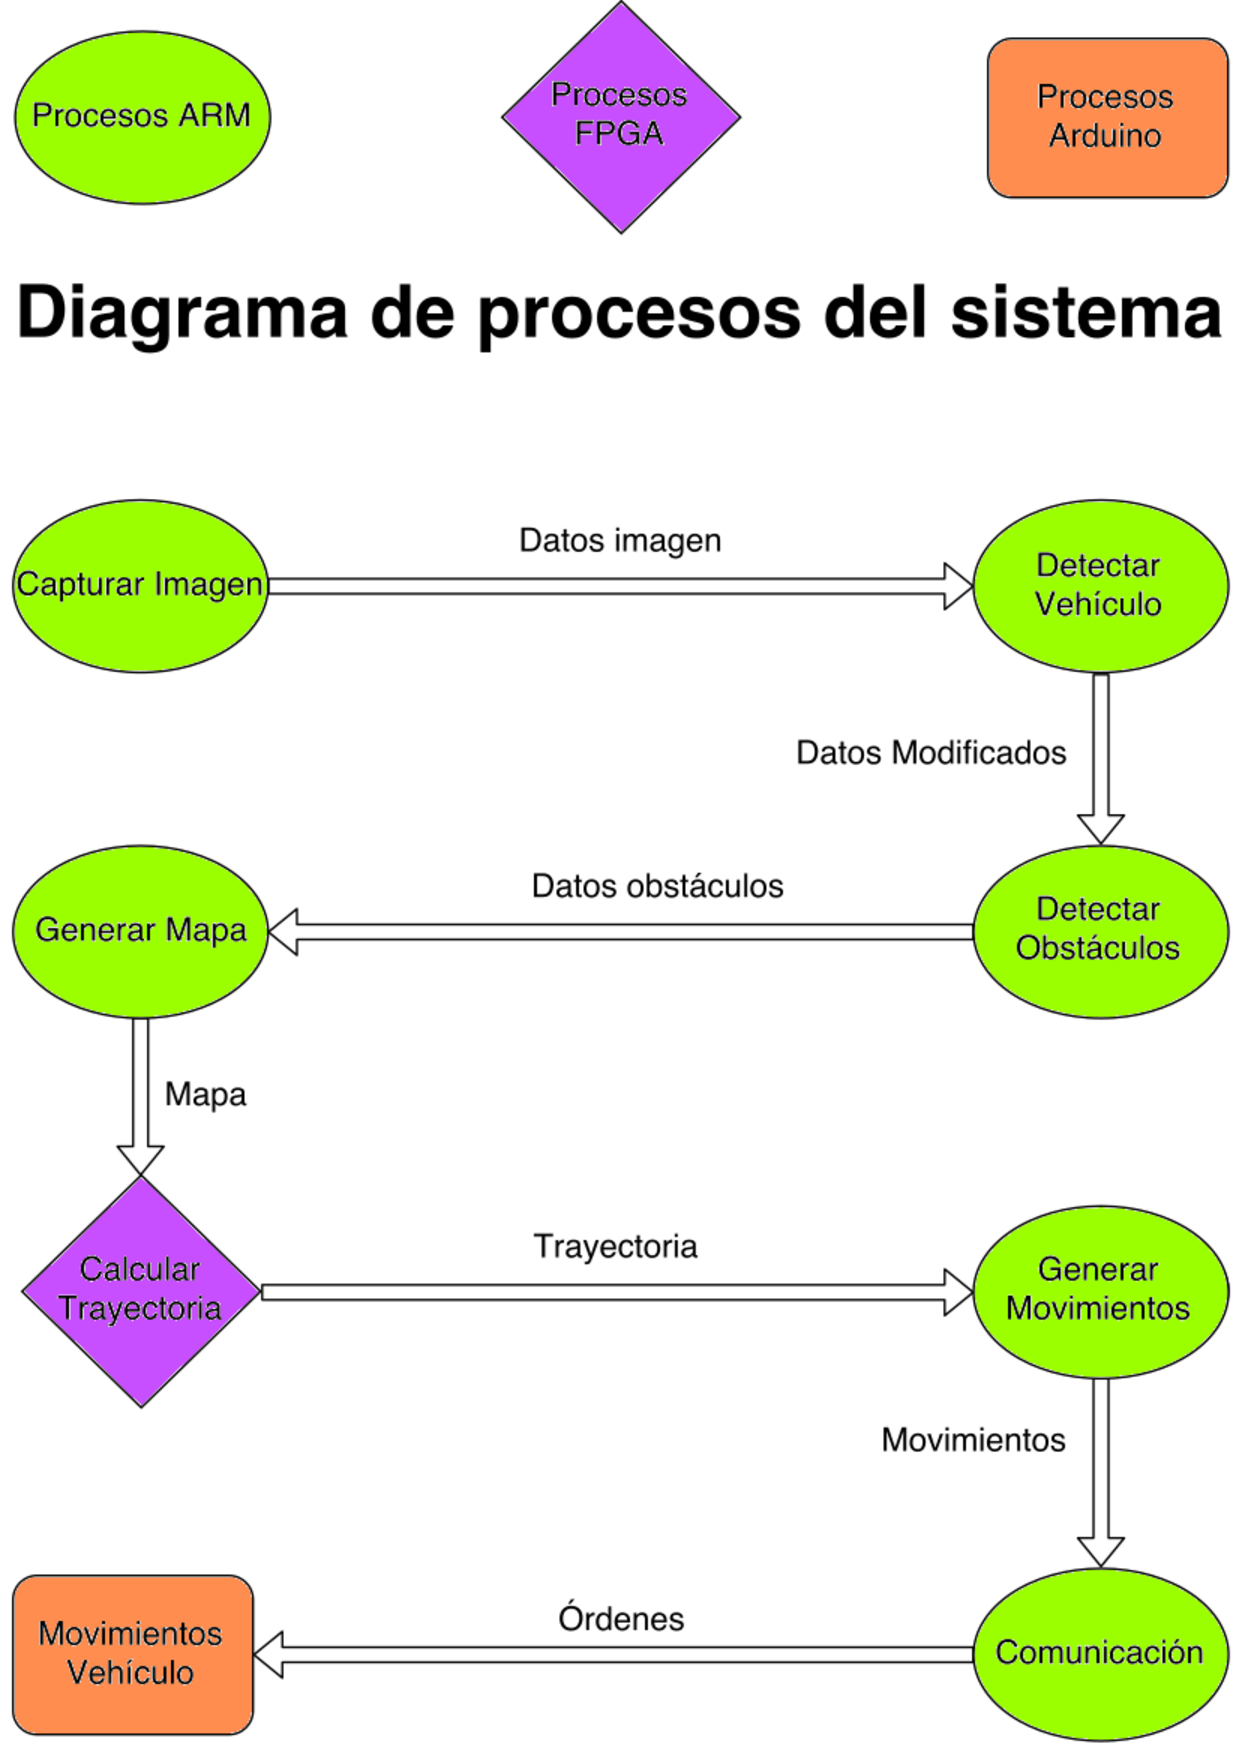
\includegraphics[width=1.11\textwidth]{./figures/DiagramaProcesos.pdf}
\end{figure}\label{fig:DiagramaProcesos}

Para realizar la integración del sistema en la placa \emph{Zedboard} se ha seguido la estructura del diagrama de procesos de la figura \ref{fig:DiagramaProcesos}. Como se puede observar se ha decidido embeber únicamente el algoritmo de cálculo de trayectoria en \ac{FPGA}. Mediante el uso de la herramienta \emph{Petalinux} se ha realizado una compilación cruzada desde un ordenador diferente a la placa. La compilación de la aplicación en el propio procesador \ac{ARM} es muy compleja. Esto es debido a que la librería \emph{OpenCV} tiene muchas dependencias en cuanto al uso de librerías externas y al utilizar un procesador \ac{ARM} tan específico el soporte de la distribución es escaso. Como solución se decidió crear un directorio sobre el cual se pudiera emular la distribución \emph{Debian} que se ha utilizado en la placa \emph{Zedboard}. De esta manera mediante el uso de un fichero \emph{Makefile} y la ayuda de la herramienta \emph{Petalinux} se puede realizar la compilación de la aplicación del sistema generando el archivo binario que se debe trasladar a la placa \emph{Zeboard} para su ejecución.

Con la herramienta \emph{Vivado} \ac{HLS} se genera el componente \ac{IP} con la funcionalidad del algoritmo A*. Este componente \ac{IP} será cargado al catálogo \ac{IP} de la herramienta \emph{Vivado} para realizar su posterior integración en la placa \emph{Zedboard}. Finalmente, con la herramienta \ac{SDK} se invocan funciones necesarias para la utilización del componente referente al algoritmo de cálculo de trayectoria.



